\documentclass[xcolor={usenames,dvipsnames,svgnames}, compress]{beamer}

\usepackage{booktabs}
\usepackage{dcolumn}
\usepackage{colortbl}
\usepackage{xcolor}
\usepackage{hyperref}
\usepackage{amsmath}
\usepackage{wrapfig}
\usepackage[style=authoryear-comp]{biblatex}

\usepackage[font=scriptsize]{caption}

%
% custom colors
\definecolor{untractable_red}{RGB}{209, 25, 25}
\definecolor{tractable_green}{RGB}{0, 153, 51}

\usetheme{enziteto}


\setbeamertemplate{headline}{}

\addbibresource{../referomnia/referomnia.bib}

\begin{document}

\newlength{\custombulletheight}
\setlength{\custombulletheight}{\dimexpr0.5\ht1-0.5\ht2}

\newcommand{\plusbullet}{\raisebox{\custombulletheight}{\hbox{\tiny\textcolor{lacamlilac}{$\boldsymbol{\oplus}$}}\hspace{-2pt}}}

\setbeamertemplate{itemize item}{\raisebox{.21ex}{\hbox{\tiny\textcolor{lacamlilac}{$\boldsymbol{\oplus}$}}\hspace{-2pt}}}
\setbeamertemplate{itemize subitem}{\raise .2ex\hbox{\tiny\textcolor{lacamlilac}{$\boldsymbol{\otimes}$}}\hspace{-3pt}}
\setbeamertemplate{itemize subsubitem}{\textcolor{lacamlilac}{$\oplus$}}
\setbeamertemplate{bibliography item}{\hspace{10pt}\raise .2ex\hbox{\tiny\textcolor{lacamlilac}{$\boldsymbol{\oplus}$}}}



% 
% custom bullets

% \renewcommand\labelitemi{\raisebox{\custombulletheight}{\hbox{\tiny\textcolor{lacamlilac}{$\boldsymbol{\oplus}$}}\hspace{-2pt}}}
\title{Simplifying, Regularizing and Strengthening Sum-Product Network Structure Learning}
\author{Antonio  Vergari, Nicola  {Di Mauro} and Floriana Esposito}
\institute{Lacam$@$DIB$@$Uniba}
\institute{Università degli Studi di Bari}
\department{Dipartimento di Informatica}
\laboratory{LACAM Laboratory}
\group{Machine Learning}
\institutelogo{
\includegraphics[width=25pt]{figures/unibaba}}
\lablogo{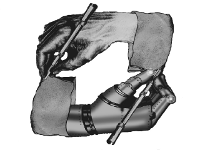
\includegraphics[width=35pt]{figures/lacam}}

\makeatletter
\defbeamertemplate*{title page}{custom-enziteto}[1][]
{
  \begin{minipage}[t]{0.1\linewidth}
    \vspace{0pt}
    % 
\includegraphics[width=25pt]{Figures/unibaba}
    \ifdefined\@institutelogo
    \@institutelogo
    \fi
  \end{minipage}
  \begin{minipage}[t]{0.28\linewidth}
    \vspace{5pt}
    \flushleft
    {\usebeamerfont{institute}\insertinstitute\par}
    \vspace{2pt}
    \ifdefined\@department
    \tiny\@department
    \fi
  \end{minipage}
  \ifdefined\@laboratory
  \hspace{15pt}
  \begin{minipage}[t]{0.12\linewidth}
    \vspace{0pt}
    \ifdefined\@lablogo
    \@lablogo
    \else
    \hspace{10pt}
    \fi
  \end{minipage}
  \begin{minipage}[t]{0.40\linewidth}
    \vspace{5pt}
    \flushleft
    \tiny\textbf{\@laboratory}\par
    \vspace{2pt}
    \ifdefined\@group
    \@group
    \fi
  \end{minipage}
  \par
  \fi
  \vspace{10pt}
  
  \Large\usebeamerfont{title}\usebeamercolor{title
    page}\inserttitle\par%\textcolor{lacamlilac}{\inserttitle}\par
  \ifdefined\@subtitle
  \vspace{5pt}
  \small\usebeamerfont{subtitle}\textcolor{lacamlilac}{\insertsubtitle}\par
  \fi
  \vspace{15pt}
  \usebeamerfont{author}\insertauthor\par
  
  \ifdefined\@gliph
  \vspace{7pt}
  \@gliph\par
  \vspace{7pt}
  \else
  \vspace{21pt}
  \fi

  {\vspace{-15pt}\usebeamerfont{author} ECML-PKDD 2015} - {\usebeamerfont{date} 7 - 11 September Porto, Portugal}
  %\usebeamerfont{date}\insertdate\par
}
\makeatother


{
  \setbeamertemplate{headline}{}
  \setbeamertemplate{footline}{}
  \begin{frame}
    \titlepage
  \end{frame}
}

% \begin{frame}
%   \frametitle{Summary}
%   \begin{itemize}
%     \itemsep 10pt
%   \item Sum-Product Networks and tractable models
%   \item How and why to perform structure learning
%   \item Simplifying by limiting node splits
%   \item Regulizing by effective early stopping
%   \item Strengthening by model averaging
%     \item Conclusions and further works
%   \end{itemize}
% \end{frame}


\begin{frame}
  \frametitle{Introduction}
  \footnotesize
  The main task on \emph{\textbf{Probabilistic Graphical Models}} (PGMs), \emph{inference}, is untractable.\par\bigskip
  
  \emph{\textbf{Tractable}} PGMs are recently gaining interest: tree based models~\emph{\parencite{Meila2000}}, Arithmetic Circuits (ACs)~\emph{\parencite{Rooshenas2014-short}},
  \emph{\textbf{Sum-Product Networks}}
  (SPNs)~\emph{\parencite{Poon2011a}}.\par\bigskip

  Sum-Product Networks structure learning: \emph{\textbf{LearnSPN}}.\par\bigskip

  Improving LearnSPN on \emph{\textbf{structure quality}} and \textbf{\emph{accuracy}}, in three ways:
  \begin{enumerate}[I]
  %\itemsep 10pt
  % \item Sum-Product Networks and tractable models
  % \item How and why to perform structure learning
  \item \textbf{simplifying} by limiting node splits 
  \item \textbf{regularizing} by effective early stopping
  \item \textbf{strengthening} by model averaging 
  \end{enumerate}
\end{frame}


\begin{frame}[t]
  \frametitle{PGMs and Tractability}
  \begin{table}[!ht]
    \setlength{\tabcolsep}{25pt}
    \centering
    \begin{tabular}{c c}
      
      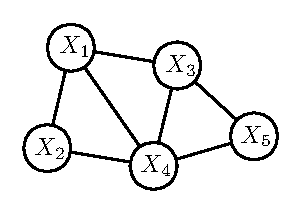
\includegraphics[width=0.33\linewidth]{figures/mrf} &
                                                            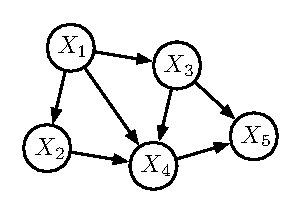
\includegraphics[width=0.33\linewidth]{figures/bn}\\
      \addlinespace[-0.2cm]
      \scriptsize  $P(\mathbf{X})=\frac{1}{Z}\prod_{c}\phi_{c}(\mathbf{X}_{c})$
                                                          & 
      \scriptsize
                                                            $P(\mathbf{X})=\prod_{i=1}^nP(X_{i}|\mathbf{Pa}_{i})$\\
      \addlinespace[0.5cm]
      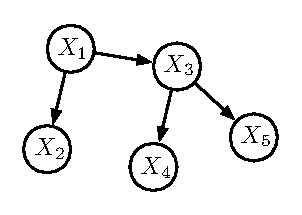
\includegraphics[width=0.33\linewidth]{figures/clt} &
                                                            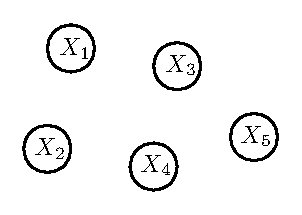
\includegraphics[width=0.33\linewidth]{figures/nf}\\
      \addlinespace[-0.2cm]
      \scriptsize
      $P(\mathbf{X})=\prod_{i=1}^nP(X_{i}|Pa_{i})$ &
      \scriptsize $P(\mathbf{X})=\prod_{i=1}^nP(X_{i})$                                                              
    \end{tabular}
  \end{table}
  %\footnotesize Inference on Probabilistic Graphical Models (PGMs) is generally untractable.
\end{frame}

\begin{frame}[t]
  \frametitle{PGMs and Tractability}
  \begin{table}[!ht]
    \setlength{\tabcolsep}{25pt}
    \centering
    \begin{tabular}{c c}
      
      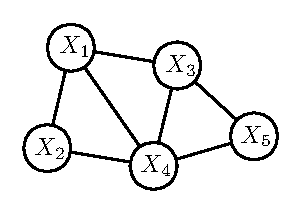
\includegraphics[width=0.33\linewidth]{figures/mrf} &
                                                            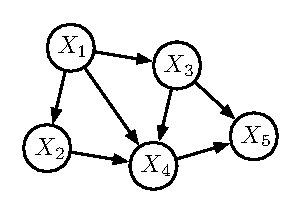
\includegraphics[width=0.33\linewidth]{figures/bn}\\
      \addlinespace[-0.2cm]
      \scriptsize\color{untractable_red}  \textbf{\emph{untractable}} & \scriptsize\color{untractable_red} \textbf{\emph{untractable}} \\
      \addlinespace[0.5cm]
      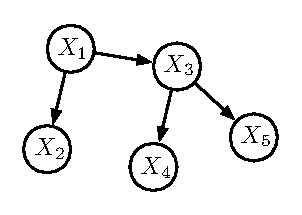
\includegraphics[width=0.33\linewidth]{figures/clt} &
                                                            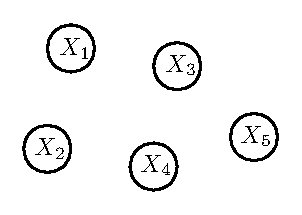
\includegraphics[width=0.33\linewidth]{figures/nf}\\
      \addlinespace[-0.2cm]
      \scriptsize\color{tractable_green} \emph{\textbf{tractable}} & \scriptsize\color{tractable_green} \emph{\textbf{tractable}}                                                              
    \end{tabular}
  \end{table}
  %\footnotesize To guarantee polynomial inference, tractable models trade off model expressiveness.
\end{frame}

\begin{frame}[t]
  \frametitle{Sum-Product Networks (I)}
  \footnotesize
   SPNs are DAGs \emph{compiling} the partition function of a joint pdf into a \textbf{\emph{deep}} architecture of \textbf{sum}
   and \textbf{product} nodes.\par\bigskip

   Product nodes define factorizations over independent components, sum
   nodes weighted mixtures. Leaves are tractable univariate distributions.\par\bigskip

   \begin{minipage}{0.45\linewidth}
    \centering
    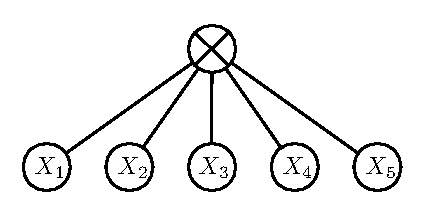
\includegraphics[width=0.72\linewidth]{figures/spn-prod}\\
    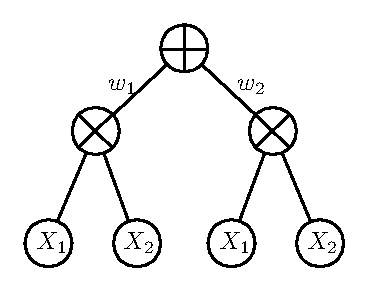
\includegraphics[width=0.653\linewidth]{figures/spn-sum}
  \end{minipage}%
  \begin{minipage}{0.5\linewidth}
    \vspace{7pt}
    % \footnotesize
    % SPNs are DAGs \emph{compiling} the partition function of a joint pdf into a \textbf{\emph{deep}} architecture of \textbf{sum}
    % and \textbf{product} nodes.\\

    % Product nodes define factorizations over independent components, sum
    % nodes mixtures. Leaves are tractable univariate distributions.\\

    %Sum node children weights are the parameters of the model.\\

    Products over nodes with different scopes (\emph{decomposability}) and
    sums over nodes with same scopes (\emph{completeness}) guarantee modeling
    a pdf (\emph{validity}).\par\bigskip

    The \emph{\textbf{size}} of the network is the number of \emph{edges} in it.\par\bigskip

    The \emph{\textbf{depth}} of the network is the number of alternated \emph{layers}.\par\bigskip

    % Considering only valid SPNs of \emph{alternated layers of sum and products}.

    

    

  \end{minipage}
\end{frame}

\begin{frame}
  \frametitle{Sum-Product Networks (II)}
  \begin{minipage}{0.35\linewidth}
    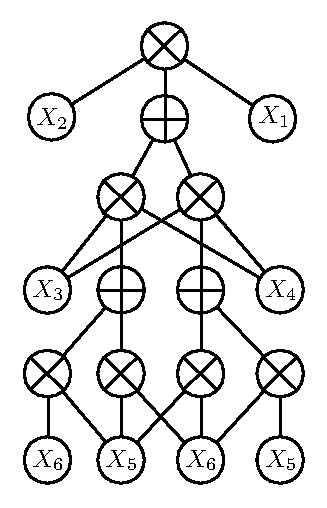
\includegraphics[width=0.9\linewidth]{figures/spn-long}
  \end{minipage}\begin{minipage}{0.62\linewidth}
    \footnotesize
    Bottom-up evaluation of the network:
    \begin{align*}
      \quad&S_{X_i}(x_j)=P(X_i=x_j)\\[10pt]
      \quad&S_{+}(\mathbf{x})=\sum\limits_{i\in
                         ch(+)}w_{i}S_{i}(\mathbf{x}),\quad S_{\times}(\mathbf{x})=\prod\limits_{i\in
      ch(\times)}S_{i}(\mathbf{x})
    \end{align*}\\[-7pt]
    
    Inferences linear in the size of the network (\# edges):\\[-5pt]
    \begin{itemize}
    \item $Z = S(*)$
    \item $P(\mathbf{e}) = S(\mathbf{e})/S(*)$
    \item $P(\mathbf{q}| \mathbf{e}) = \frac{P(\mathbf{q},
        \mathbf{e})}{P(\mathbf{e})} = \frac{S(\mathbf{q},
        \mathbf{e})}{S(\mathbf{e})}$
    \item $MPE(\mathbf{q},\mathbf{e}) = \max_{\mathbf{q}}P(\mathbf{q},
      \mathbf{e}) = S^{max}(\mathbf{e})$  (by substituting sum nodes
      with \emph{max} nodes)
    \end{itemize}
     
    
    
  \end{minipage}
\end{frame}

\begin{frame}
  \frametitle{How and Why Structure Learning}
  \footnotesize
  Fixed structures are hard to engineer and train (fully connected layers).\par\bigskip
  
  Automatic discovery of latent vars.\par\bigskip

   \emph{Constraint-based search} formulation. Discover hidden variables for sum node mixtures and independences
  for product node components:
  \begin{itemize}
    \itemsep 6pt
  \item greedy top-down: KMeans on features~\emph{\parencite{Dennis2012}}; alternating clustering on
    instances and independence tests on features, \textbf{LearnSPN}~\emph{\parencite{Gens2013}}

  \item greedy bottom up: merging feature regions by a \emph{Bayesian-Dirichlet independence test},  and reducing edges by maximizing MI\emph{~\parencite{Peharz2013}}

  

  \item \textbf{ID-SPN}: turning LearnSPN in log-likelihood guided expansion of sub-networks
    approximated by Arithmetic Circuits~\emph{\parencite{Rooshenas2014-short}}

  \end{itemize}
  \vspace{6pt}

  
\end{frame}

\begin{frame}
  \frametitle{Why Structure Quality Matters}

  \footnotesize
  
  Tractable inference is guaranteed \emph{if the network size is polynomial} in \#
  vars.\par\bigskip

  Smaller networks, faster inference (comparing network sizes is better than comparing inference times).\par\bigskip

  \emph{Deeper} networks are possibly \emph{more expressively efficient}~\emph{\parencite{Martens2014,Zhao2015}}.\par\bigskip

  Structural simplicity as a bias: overcomplex networks may not generalize well.\par\bigskip
  
  Structure quality desiderata: \textbf{\textbf{smaller}} but \textbf{\textbf{accurate}}, \textbf{\emph{deeper}} but not
  wider, SPNs.

  
  
\end{frame}

\begin{frame}[t]
  \frametitle{LearnSPN (I)}
  \footnotesize
  Build a tree-like SPN by recursively split the data matrix:

  \begin{itemize}
  \item splitting columns into pairs by a greedy \textbf{\emph{G Test}} based
    procedure with threshold $\rho$:
    \[
    G(X_i, X_j) =  2\sum_{x_i \sim X_i}\sum_{x_j \sim X_j}c(x_i, x_j)\cdot \log\frac{c(x_i, x_j)\cdot |T|}{c(x_i)c(x_j)}
    \]
  \item clustering instances into $|C|$ sets with \textbf{\emph{online Hard-EM}} with cluster penalty
    $\lambda$:
    \[\begin{array}{cc}
        Pr(\mathbf{X})= \sum_{C_i \in \mathbf{C}}\prod_{X_j \in \mathbf{X}}Pr(X_j|C_i)Pr(C_i)\\
        % & Pr(C_i) \propto e^{-\lambda |\mathbf{C}|\cdot |\mathbf{X}|}\\
      \end{array}\]
      weights are estimated as cluster proportions
  \item if there are less than $m$ instances, put a \textbf{\emph{naive
    factorization}} over leaves
  \item each univariate distribution get \emph{\textbf{ML estimation}} smoothed by $\alpha$  
  \end{itemize}\par\bigskip

  Hyperparameter space: $\{\rho, \lambda, m, \alpha\}$.
  

\end{frame}

\begin{frame}
  \frametitle{LearnSPN (I)}
  \footnotesize
  \onslide<1-4>{\begin{minipage}[t]{0.3\linewidth}
      \begin{center}
        \only<1>{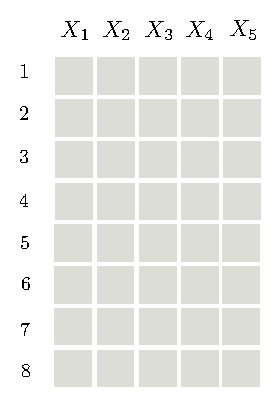
\includegraphics[width=0.8\linewidth]{figures/grid-0}}
        \only<2-4>{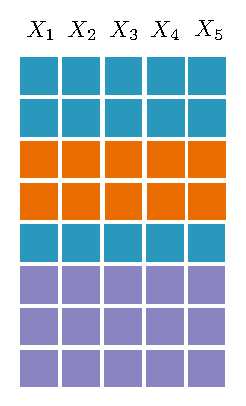
\includegraphics[width=0.715\linewidth]{figures/grid-1}}
      \end{center}
    \end{minipage}}\hspace{10pt}\onslide<3-4>{\begin{minipage}[t]{0.3\linewidth}
      \begin{center}
        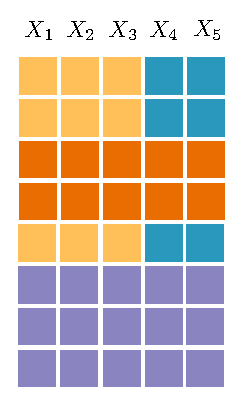
\includegraphics[width=0.72\linewidth]{figures/grid-2}
      \end{center}
    \end{minipage}}\hspace{10pt}\onslide<4>{\begin{minipage}[t]{0.3\linewidth}
      \begin{center}
        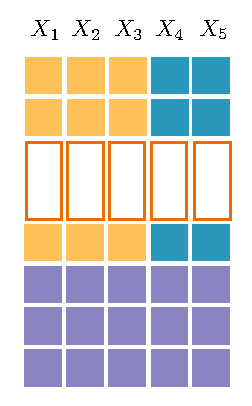
\includegraphics[width=0.735\linewidth]{figures/grid-3}
      \end{center}
    \end{minipage}}\\
  \vspace{15pt}
  \onslide<2-4>{\raisebox{0pt}{\begin{minipage}[t]{0.3\linewidth}
        \begin{center}
          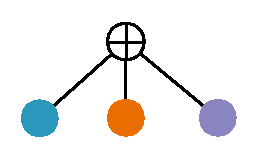
\includegraphics[width=0.715\linewidth]{figures/learnspn-1}
        \end{center}
      \end{minipage}}}\hspace{5pt}\onslide<3-4>{\raisebox{-25pt}{\begin{minipage}[t]{0.3\linewidth}
        \begin{center}
          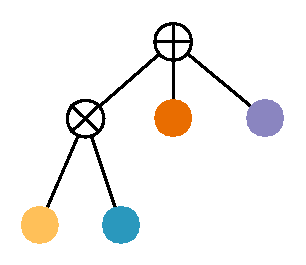
\includegraphics[width=0.83\linewidth]{figures/learnspn-2}
        \end{center}
      \end{minipage}}}\hspace{4pt}\onslide<4>{\raisebox{-22pt}{\begin{minipage}[t]{0.3\linewidth}
        \begin{center}
          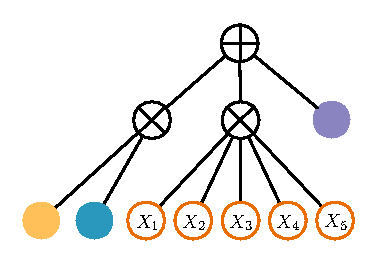
\includegraphics[width=1.0\linewidth]{figures/learnspn-3}
        \end{center}
      \end{minipage}}}
\end{frame}

% \begin{frame}

%  \onslide<1-4>{\begin{minipage}[t]{0.3\linewidth}
%      \begin{center}
%        \only<1>{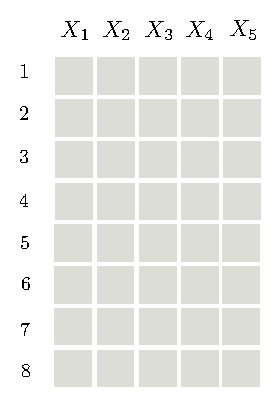
\includegraphics[width=0.8\linewidth]{figures/grid-0}}
%       \only<2-4>{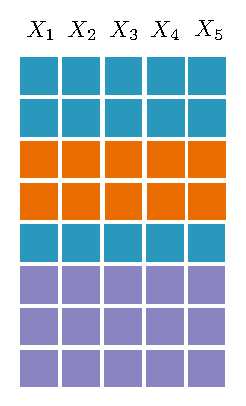
\includegraphics[width=0.715\linewidth]{figures/grid-1}}
%     \end{center}
%   \end{minipage}}\hspace{10pt}\onslide<3-4>{\begin{minipage}[t]{0.3\linewidth}
%     \begin{center}
%       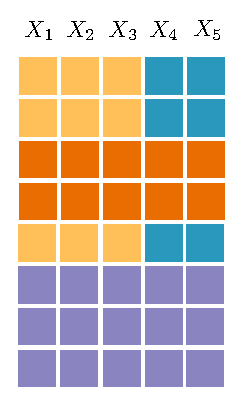
\includegraphics[width=0.72\linewidth]{figures/grid-2}
%     \end{center}
%   \end{minipage}}\hspace{10pt}\onslide<4>{\begin{minipage}[t]{0.3\linewidth}
%     \begin{center}
%       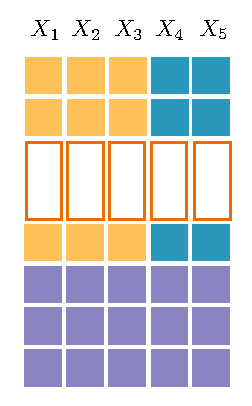
\includegraphics[width=0.735\linewidth]{figures/grid-3}
%     \end{center}
%   \end{minipage}}\\
%   \vspace{15pt}
%   \onslide<2-4>{\raisebox{0pt}{\begin{minipage}[t]{0.3\linewidth}
%     \begin{center}
%       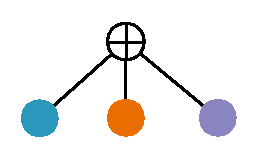
\includegraphics[width=0.715\linewidth]{figures/learnspn-1}
%     \end{center}
%   \end{minipage}}}\hspace{5pt}\onslide<3-4>{\raisebox{-25pt}{\begin{minipage}[t]{0.3\linewidth}
%     \begin{center}
%       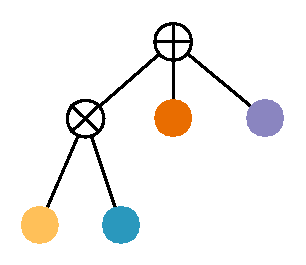
\includegraphics[width=0.83\linewidth]{figures/learnspn-2}
%     \end{center}
%   \end{minipage}}}\hspace{4pt}\onslide<4>{\raisebox{-22pt}{\begin{minipage}[t]{0.3\linewidth}
%     \begin{center}
%       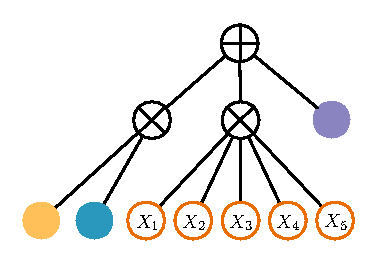
\includegraphics[width=1.0\linewidth]{figures/learnspn-3}
%     \end{center}
%   \end{minipage}}}
% \end{frame}

\begin{frame}
  \frametitle{LearnSPN (II)}
  \footnotesize
  
  \textsf{LearSPN} performs two interleaved \textbf{\emph{greedy
      hierarchical}} divisive \textbf{\emph{clustering}}
  processes (co-clutering on the data matrix).\par\bigskip

  Fast and simple. But both processes never look back and are
  committed to the choices they take.\par\bigskip

  Online EM does not need to specify the number of clusters $k$ in
  advance. But overcomplex structures are learned by exploding the number of sum
  node children.\par\bigskip

  Tractable leaf estimation. But naive factorization independence
  assumptions may be too strong.\par\bigskip

  ML estimations are effective. But they are not robust to noise, they can overfit the training set easily.
  
  \end{frame}

\begin{frame}
  \frametitle{Simplifying by limiting node splits}
  \footnotesize
  % \textsf{LearSPN} performs two interleaved \textbf{\emph{greedy
  %     hierarchical}} divisive \textbf{\emph{clustering}}
  % processes (co-clustering).\par\bigskip

  Observation: each clustering process benefits from the other one improvements/highly suffers
  from other's mistakes.\par\bigskip

  Idea: slowing down the processes by limiting the number of
  nodes to split into. \textsf{SPN-B}, variant of \textsf{LearnSPN} that uses EM
  for mixture modeling with
  $k=2$ to cluster rows.

  No need for $\lambda$ anymore.\par\bigskip

  \raisebox{45pt}{\begin{minipage}[t]{0.65\linewidth}
    Objectives:
    \begin{itemize}
    \item not committing to complex structures too early
    \item same expressive power as LearnSPN
    \item reducing node out fan increases the depth
    \item same accuracy, smaller networks
    \end{itemize}
  \end{minipage}}\hspace{-5pt}\begin{minipage}[t]{0.3\linewidth}
    \begin{center}
      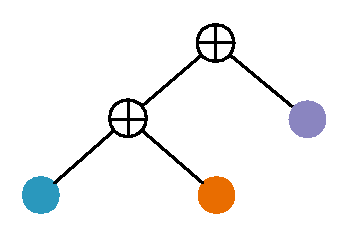
\includegraphics[width=0.9\linewidth]{figures/learnspn-4.pdf}
    \end{center}
  \end{minipage}
\end{frame}

\begin{frame}
  \frametitle{SPN-B: depth VS size}
%   \begin{table}[ht]
%     \centering
%     \begin{tabular}{c c}
%       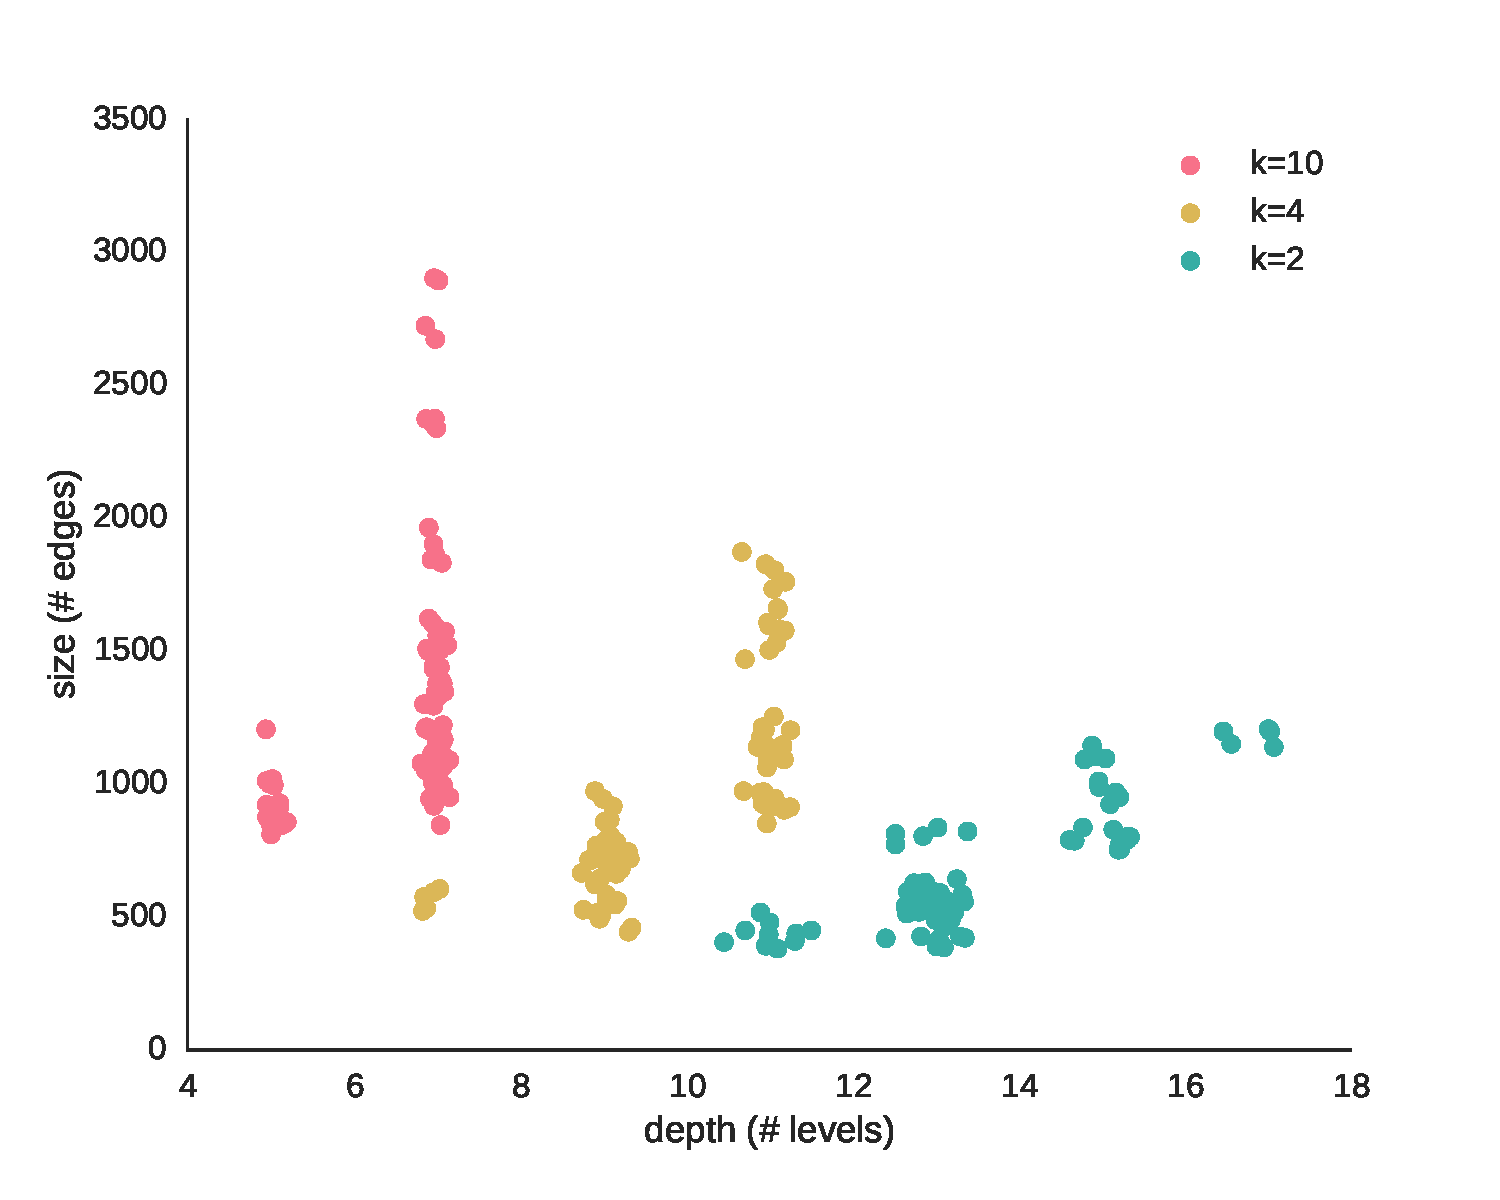
\includegraphics[width=0.45\linewidth]{figures/nltcs-depth.pdf}&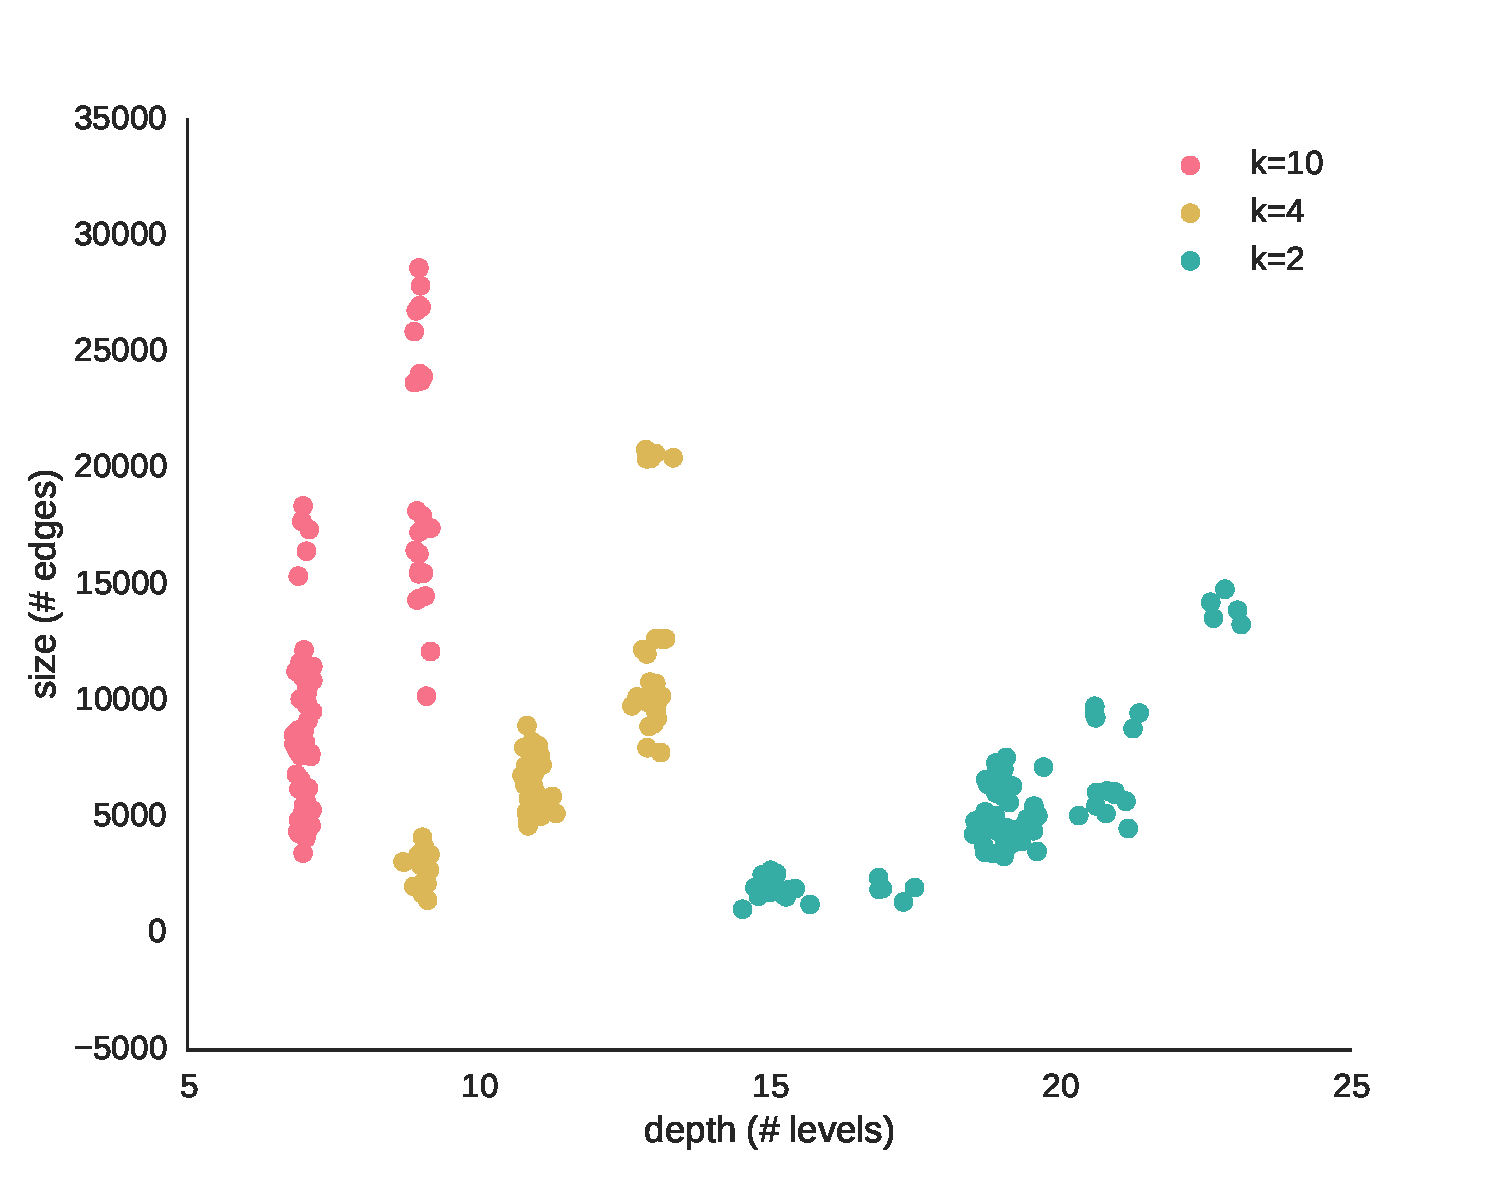
\includegraphics[width=0.45\linewidth]{figures/plants-depth.pdf}
%     \end{tabular}
%   \end{table}

  \begin{figure}[htbp]
    \begin{center}
      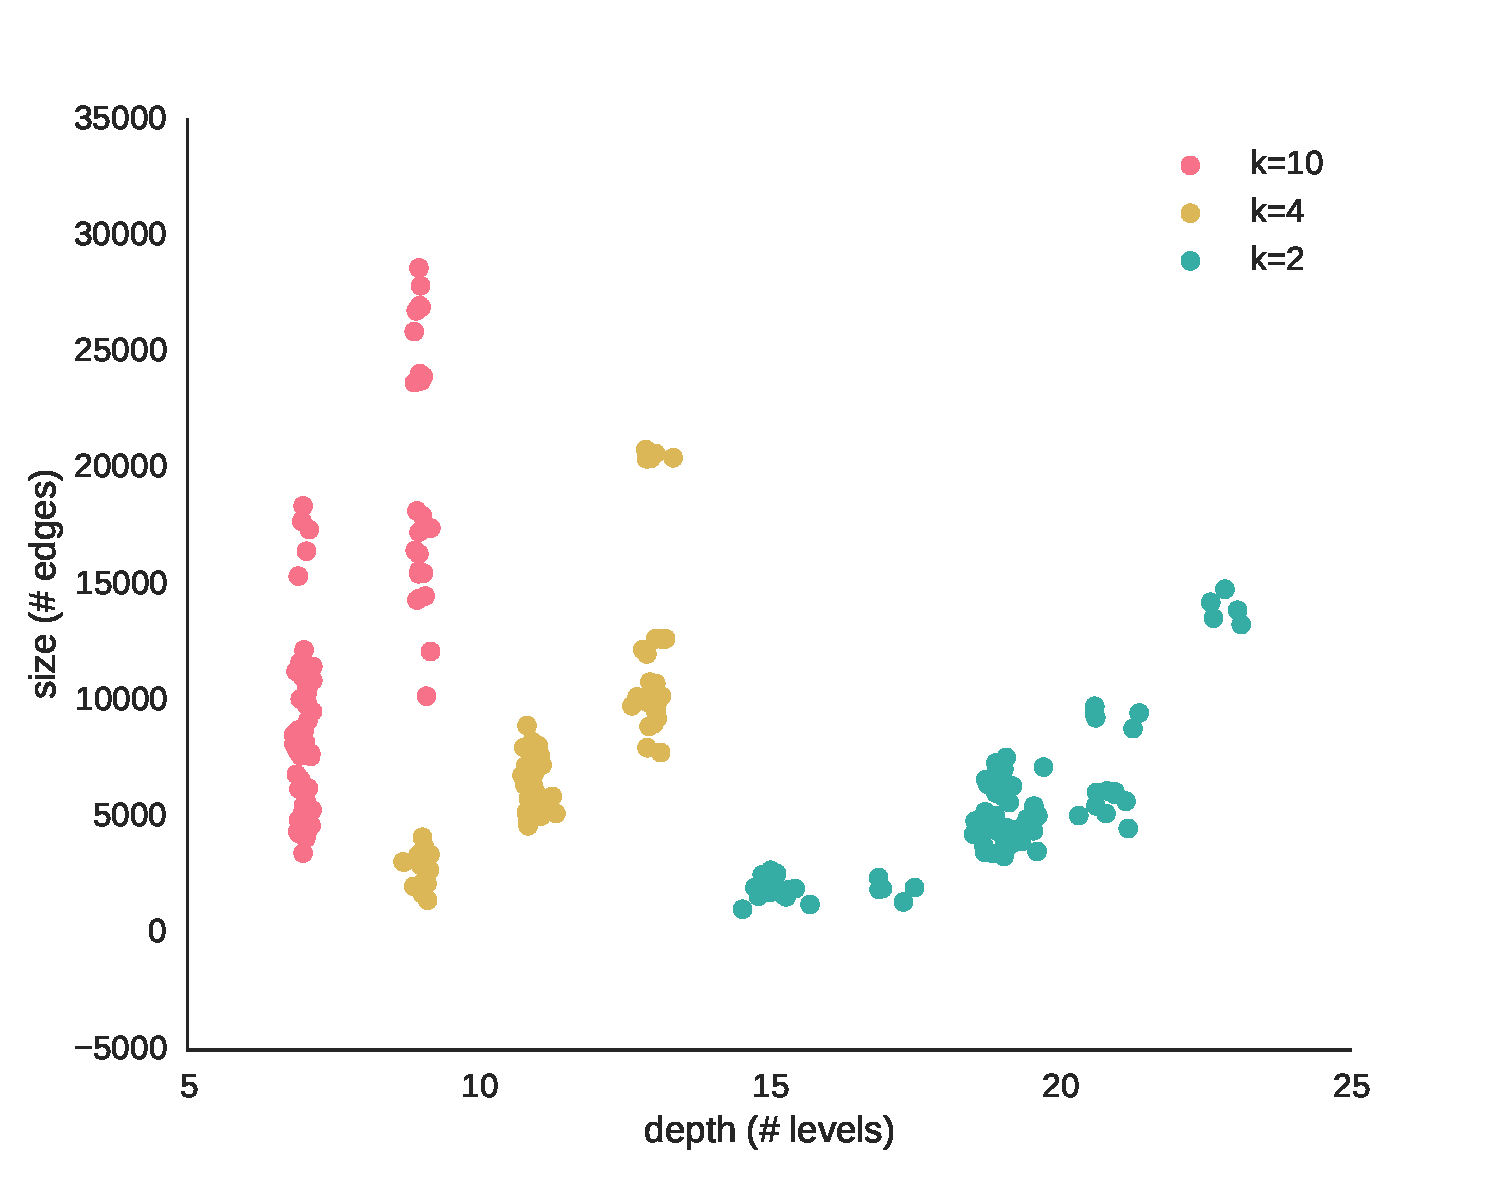
\includegraphics[width=0.6\linewidth]{figures/plants-depth.pdf}
      \caption{Comparing network sizes and depths while varying the max
        number of sum node children splits ($k\in\{10, 4, 2\}$). Each dot is an experiment
        in the grid search hyperparameter space performed by
        \textsf{SPN-B} on the dataset Plants.}
    \end{center}
  \end{figure}

\end{frame}


\begin{frame}
  \frametitle{Regularizing by effective early stopping}
  \footnotesize
  LearnSPN regularization is governed by $\alpha$ and $m$, however can
  be very ineffective:
  \begin{itemize}
  \item naive factorizations are too strong assumptions
    \item best likelihood structures prefer smaller values for $m$ to
      get accurate naive factorizations
    \end{itemize}\bigskip
    
    
    Idea: substituting naive factorizations with Bayesian trees as leaf
    distributions $P(\mathbf{X}) = \prod_{j}P(X_j|Pa_{j})$:
    \begin{wrapfigure}{l}{0.35\textwidth}
      \vspace{-20pt}
      \begin{center}
        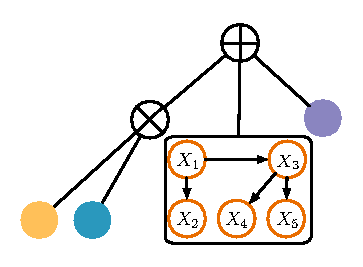
\includegraphics[width=0.35\textwidth]{figures/spn-clt}
      \end{center}
      \vspace{-20pt}
    \end{wrapfigure}
    \begin{itemize}
    \item learnable with Chow-Liu algorithm
    \item still tractable (linear) multivariate distributions for marginals,
      conditionals and MPE
    \item same or higher accuracy
    \item less complex structures for larger values of $m$
    \end{itemize}
\end{frame}

\begin{frame}
  \frametitle{SPN-BT: preserving likelihoods}

  \begin{figure}[htbp]
    \begin{center}
      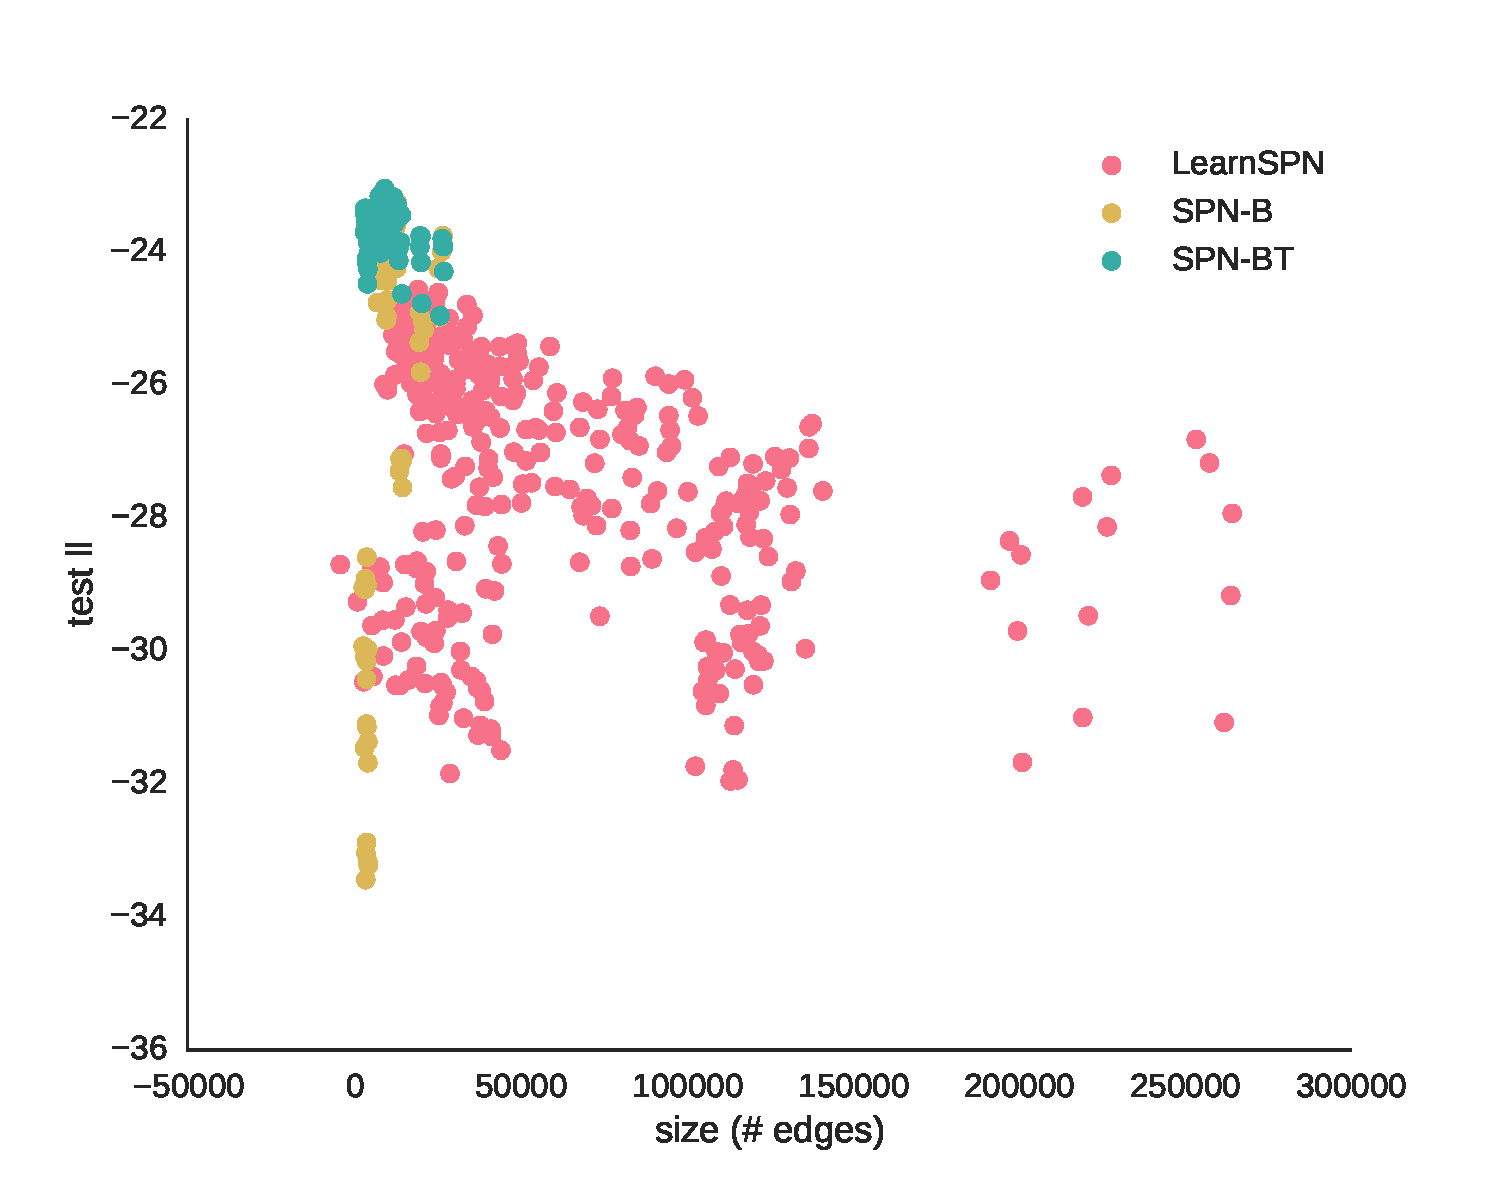
\includegraphics[width=0.7\linewidth]{figures/ll-depth/10-8/pumsb-star-ll-depth}
      \caption{Comparing the network sizes against
        the average test log-likelihood obtained by \textsf{LearnSPN},
        \textsf{SPN-B} and \textsf{SPN-BT}. Each dot is an experiment
        in the grid search performed for the dataset Pumsb-star.}
    \end{center}
  \end{figure}

\end{frame}


\begin{frame}
  \frametitle{SPN-BT: effective early stopping}
  % \begin{table}[ht]
  %   \centering
  %   \begin{tabular}{c c}
  %     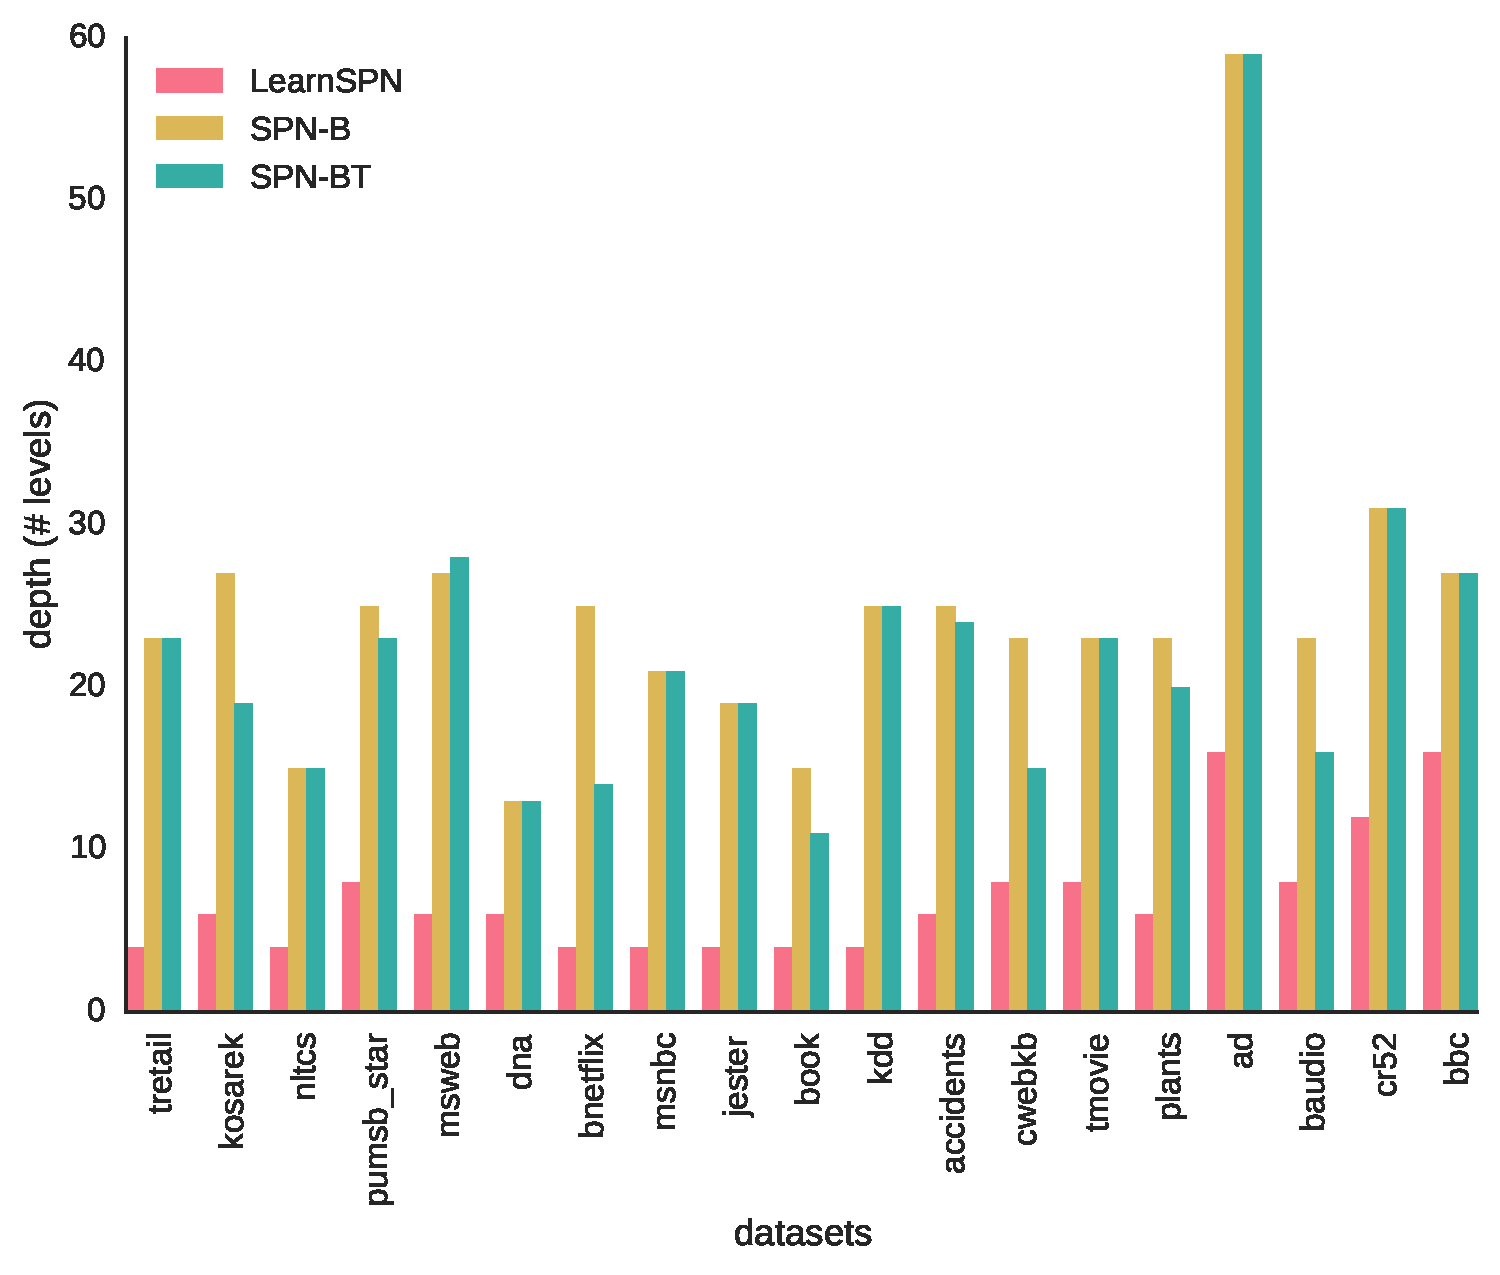
\includegraphics[width=0.45\linewidth]{figures/levels-comp}&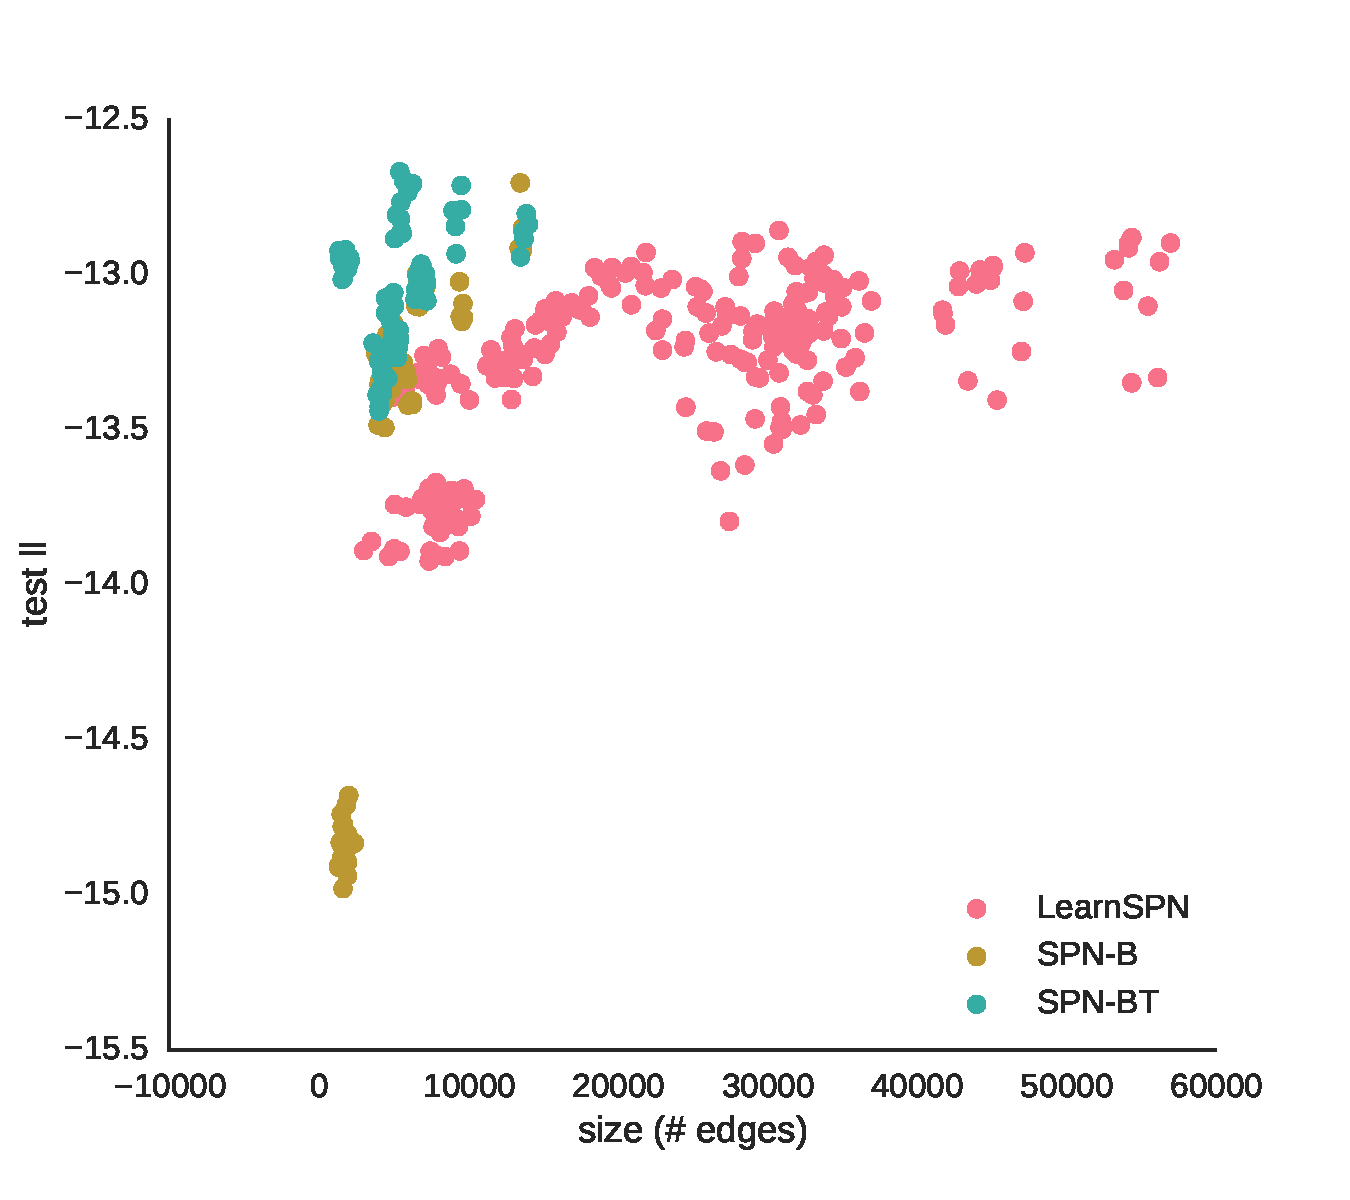
\includegraphics[width=0.45\linewidth]{figures/plants-ll-depth}
  %   \end{tabular}
  % \end{table}
  \begin{figure}[htbp]
    \begin{center}
      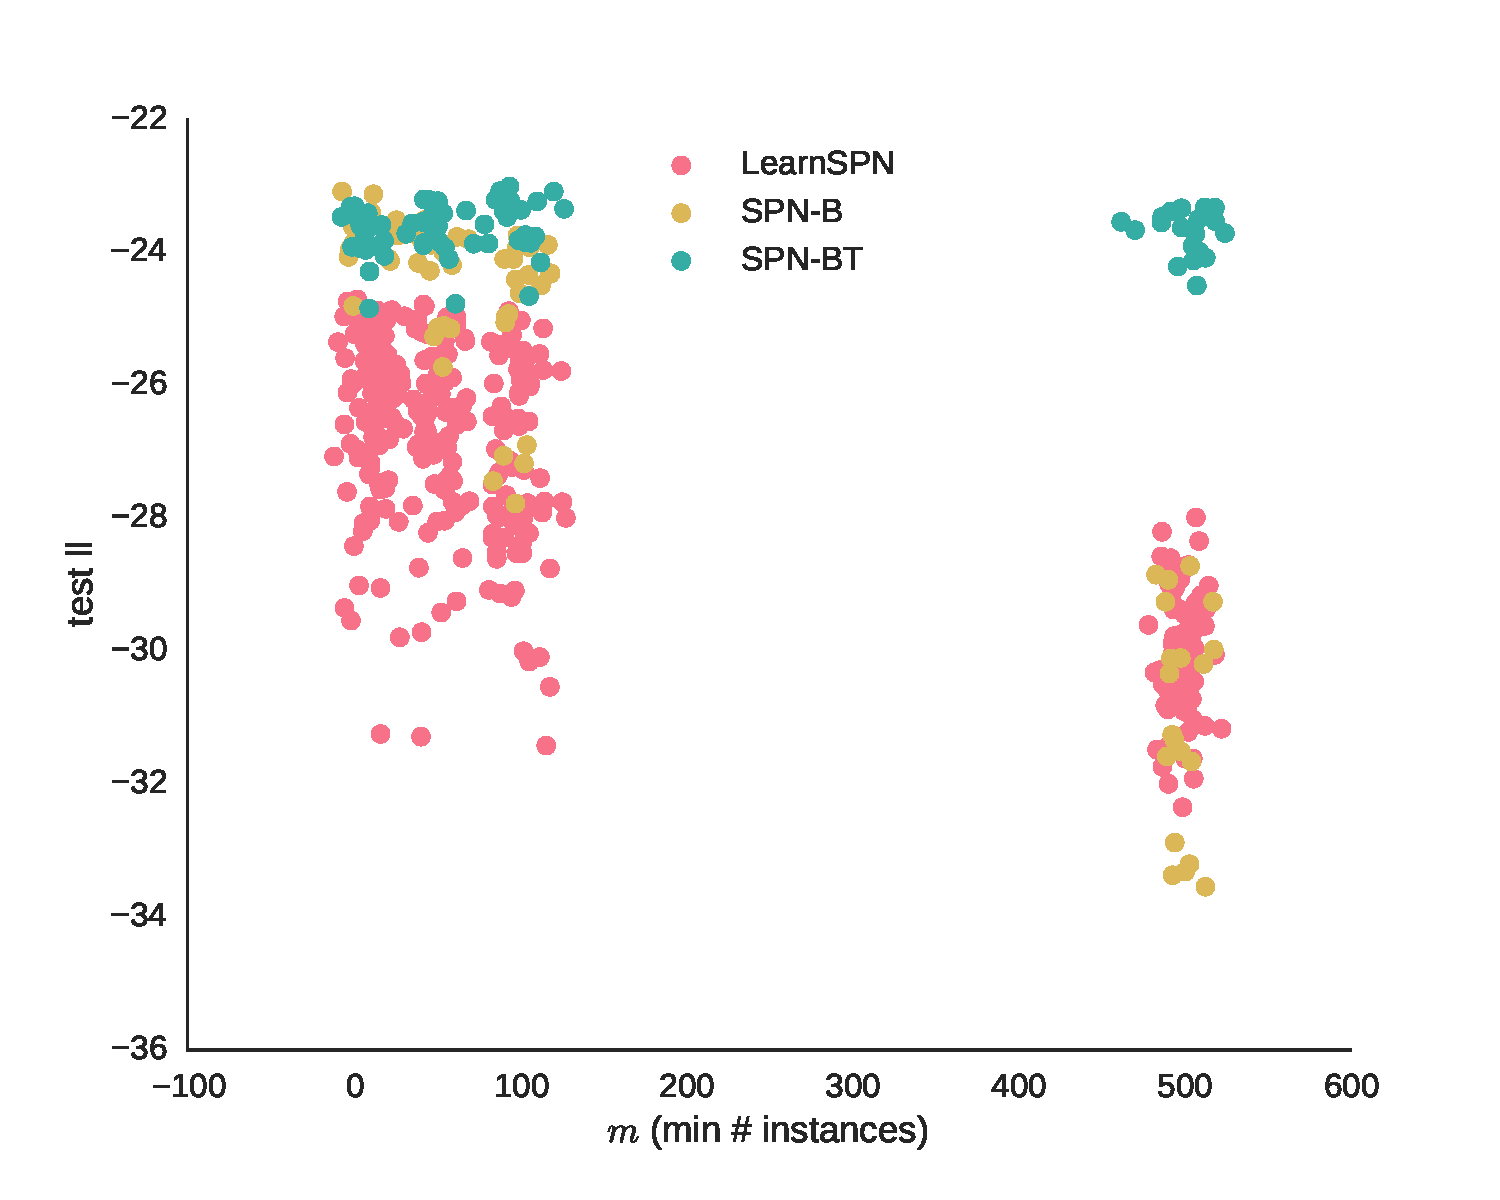
\includegraphics[width=0.7\linewidth]{figures/ll-m/10-8/pumsb-star-ll-m}
      \caption{Comparing the values for $m$ (10, 50, 100, 500) against
        the average test log-likelihood obtained by \textsf{LearnSPN},
        \textsf{SPN-B} and \textsf{SPN-BT}. Each dot is an experiment
        in the grid search performed for the dataset Pumsb-star.}
    \end{center}
  \end{figure}

\end{frame}

\begin{frame}
  \frametitle{Strengthening by model averaging}
  \footnotesize
  Interpreting sum nodes as \emph{general additive estimators}. Leveraging
  classic statistical tools to learn them:
  \textbf{\emph{bagging}}.\par\bigskip

  Draw $k$ bootstrapped samples from the data, then grow an SPN $S_{B_i}$ on
  each of them. Join them into a single SPN $\hat{S}$ with a sum node:
  $$\hat{S}=\sum_{i=1}^{k}\frac{1}{k}S_{B_{i}}$$

  More robustness and less variance in the model.\par\bigskip

  Exponential number of nodes if done for each sum node (bootstrapping
  only at the root).\par\bigskip

  Two variants in the experiments: \textsf{SPN-BB} and
  \textsf{SPN-BTB}, whether Chow-Liu trees are employed or not.
\end{frame}

\begin{frame}
  \frametitle{Bagging exp}
  \begin{table}[ht]
    \setlength{\tabcolsep}{2pt}  
    \centering
    \begin{tabular}[t]{c c}
      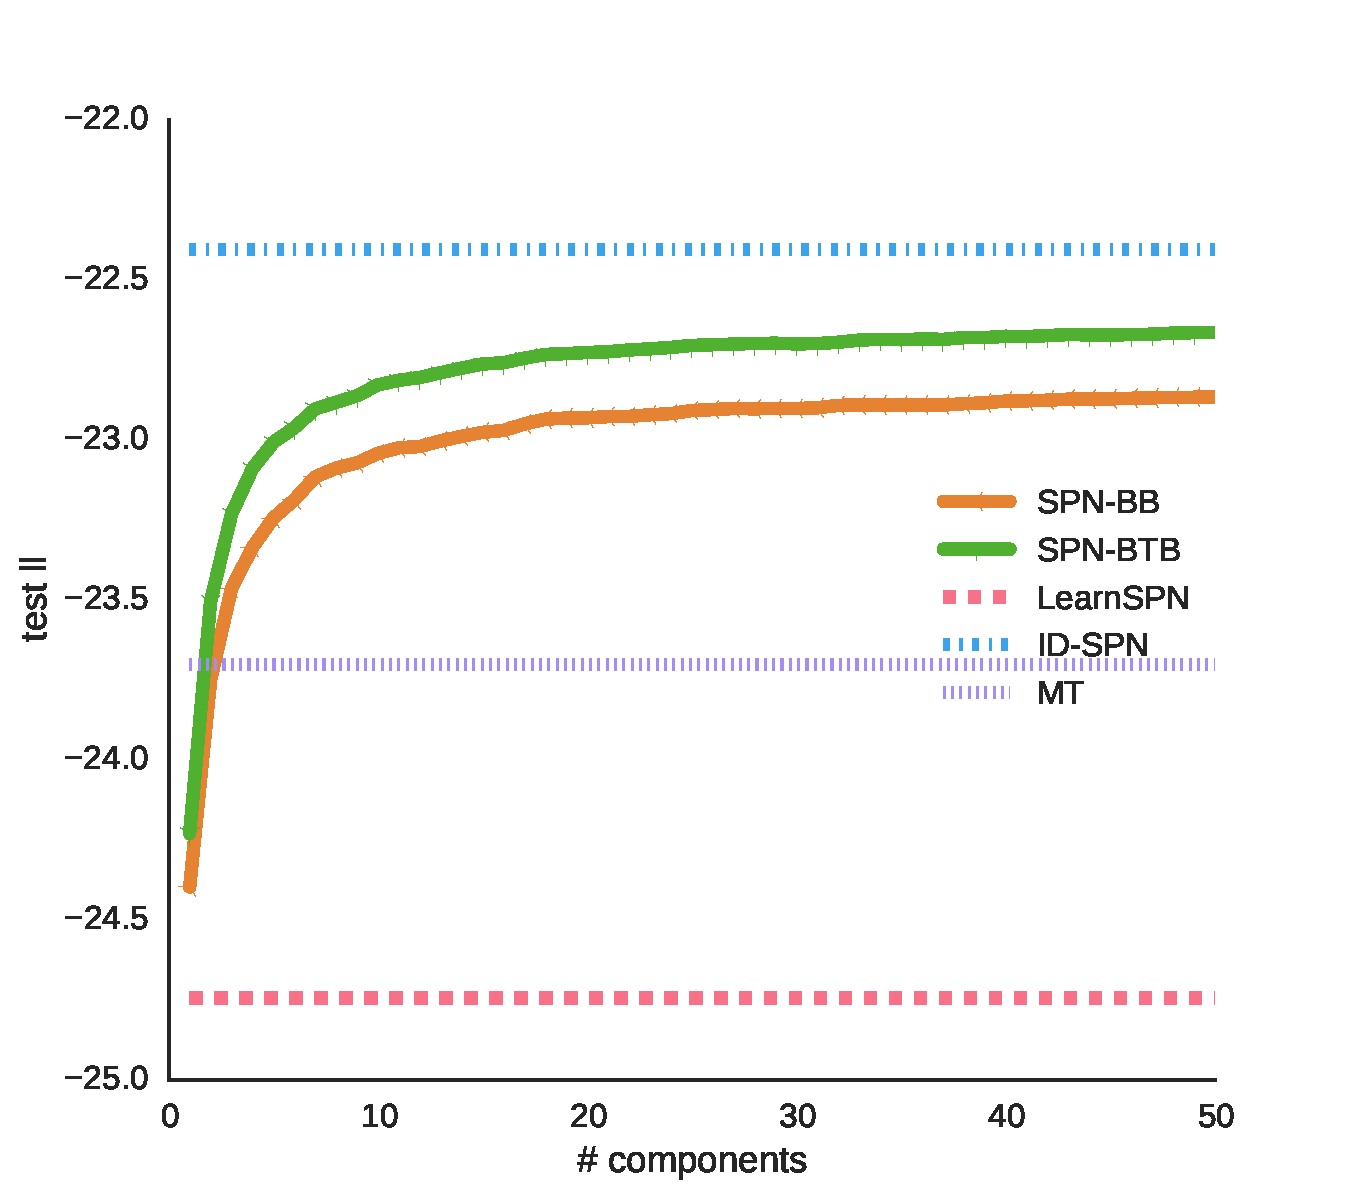
\includegraphics[width=0.5\linewidth]{figures/curves/pumsb-star-png.pdf}&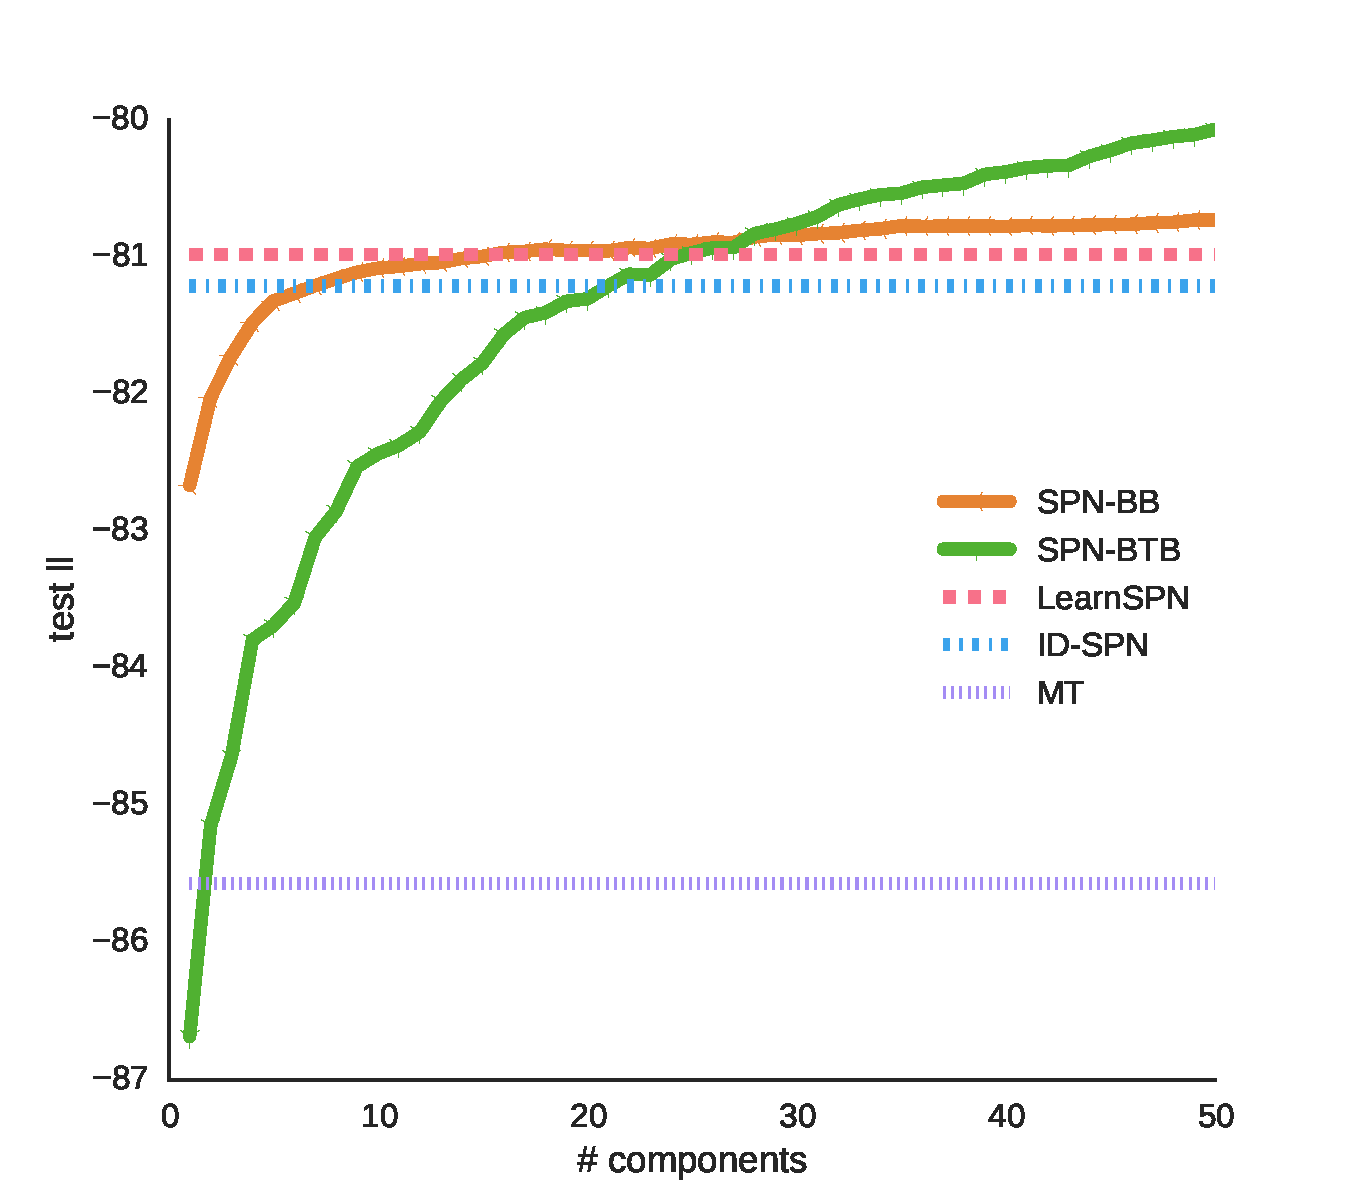
\includegraphics[width=0.5\linewidth]{figures/curves/dna-png.pdf}\\
      % 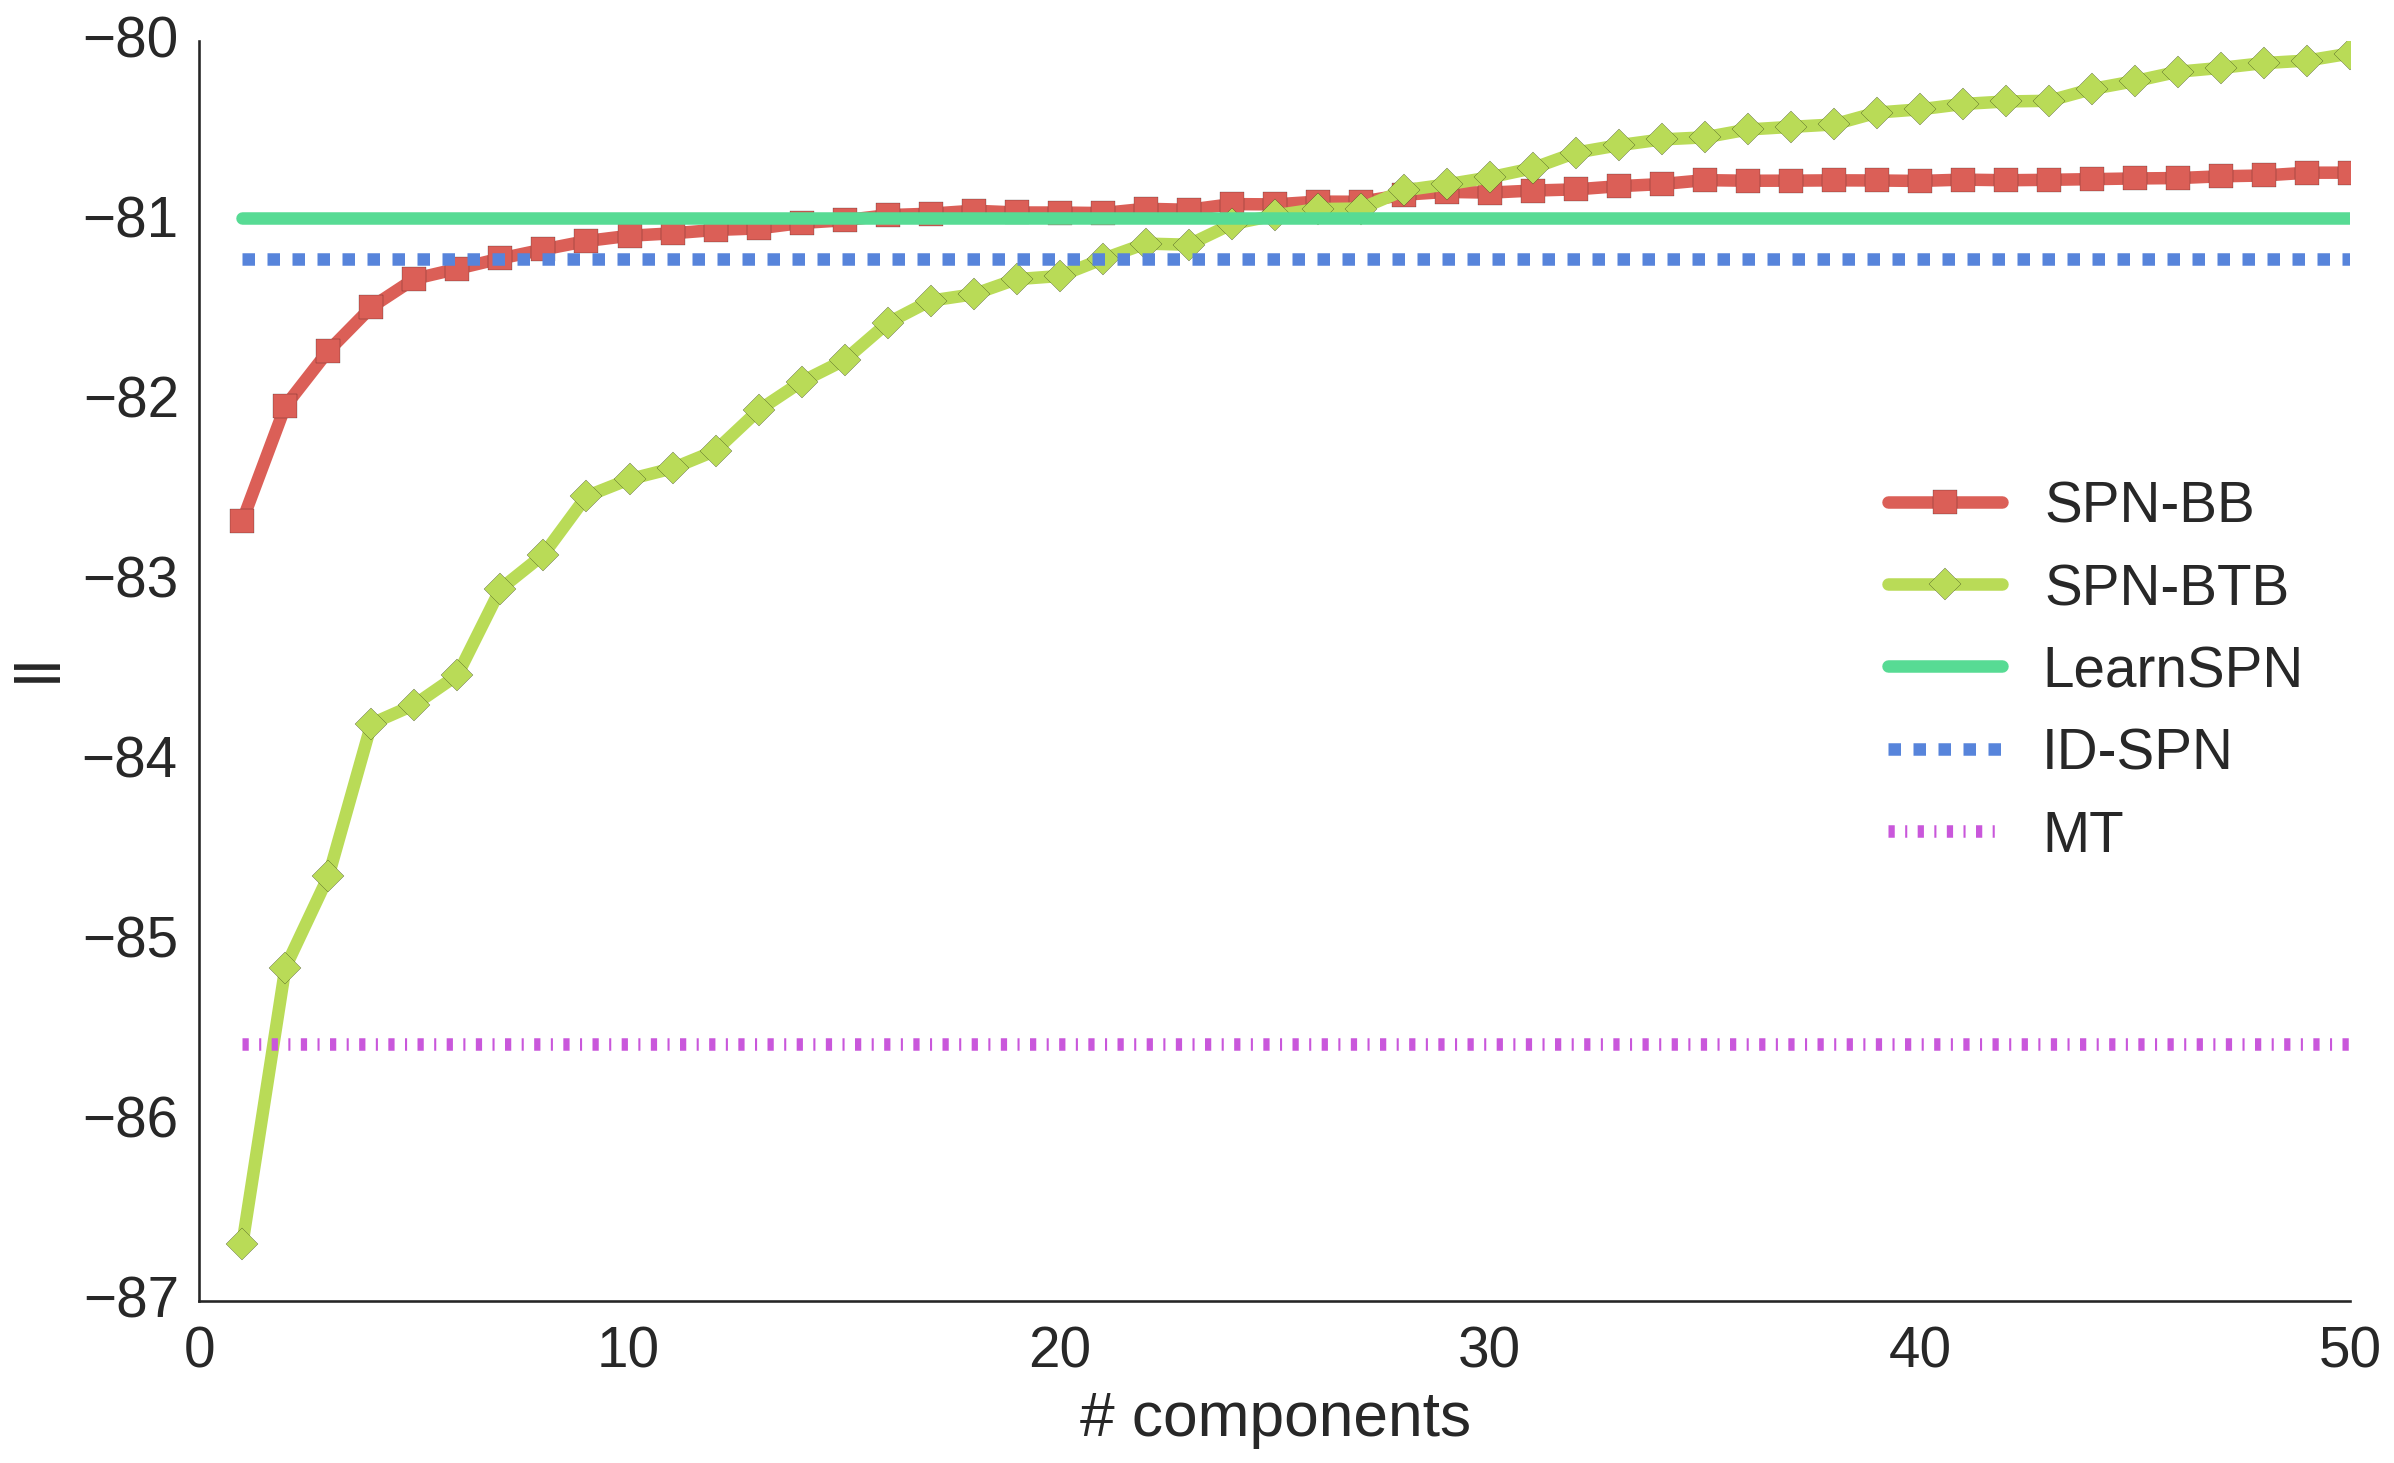
\includegraphics[width=0.4\linewidth]{figures/curves/dna}&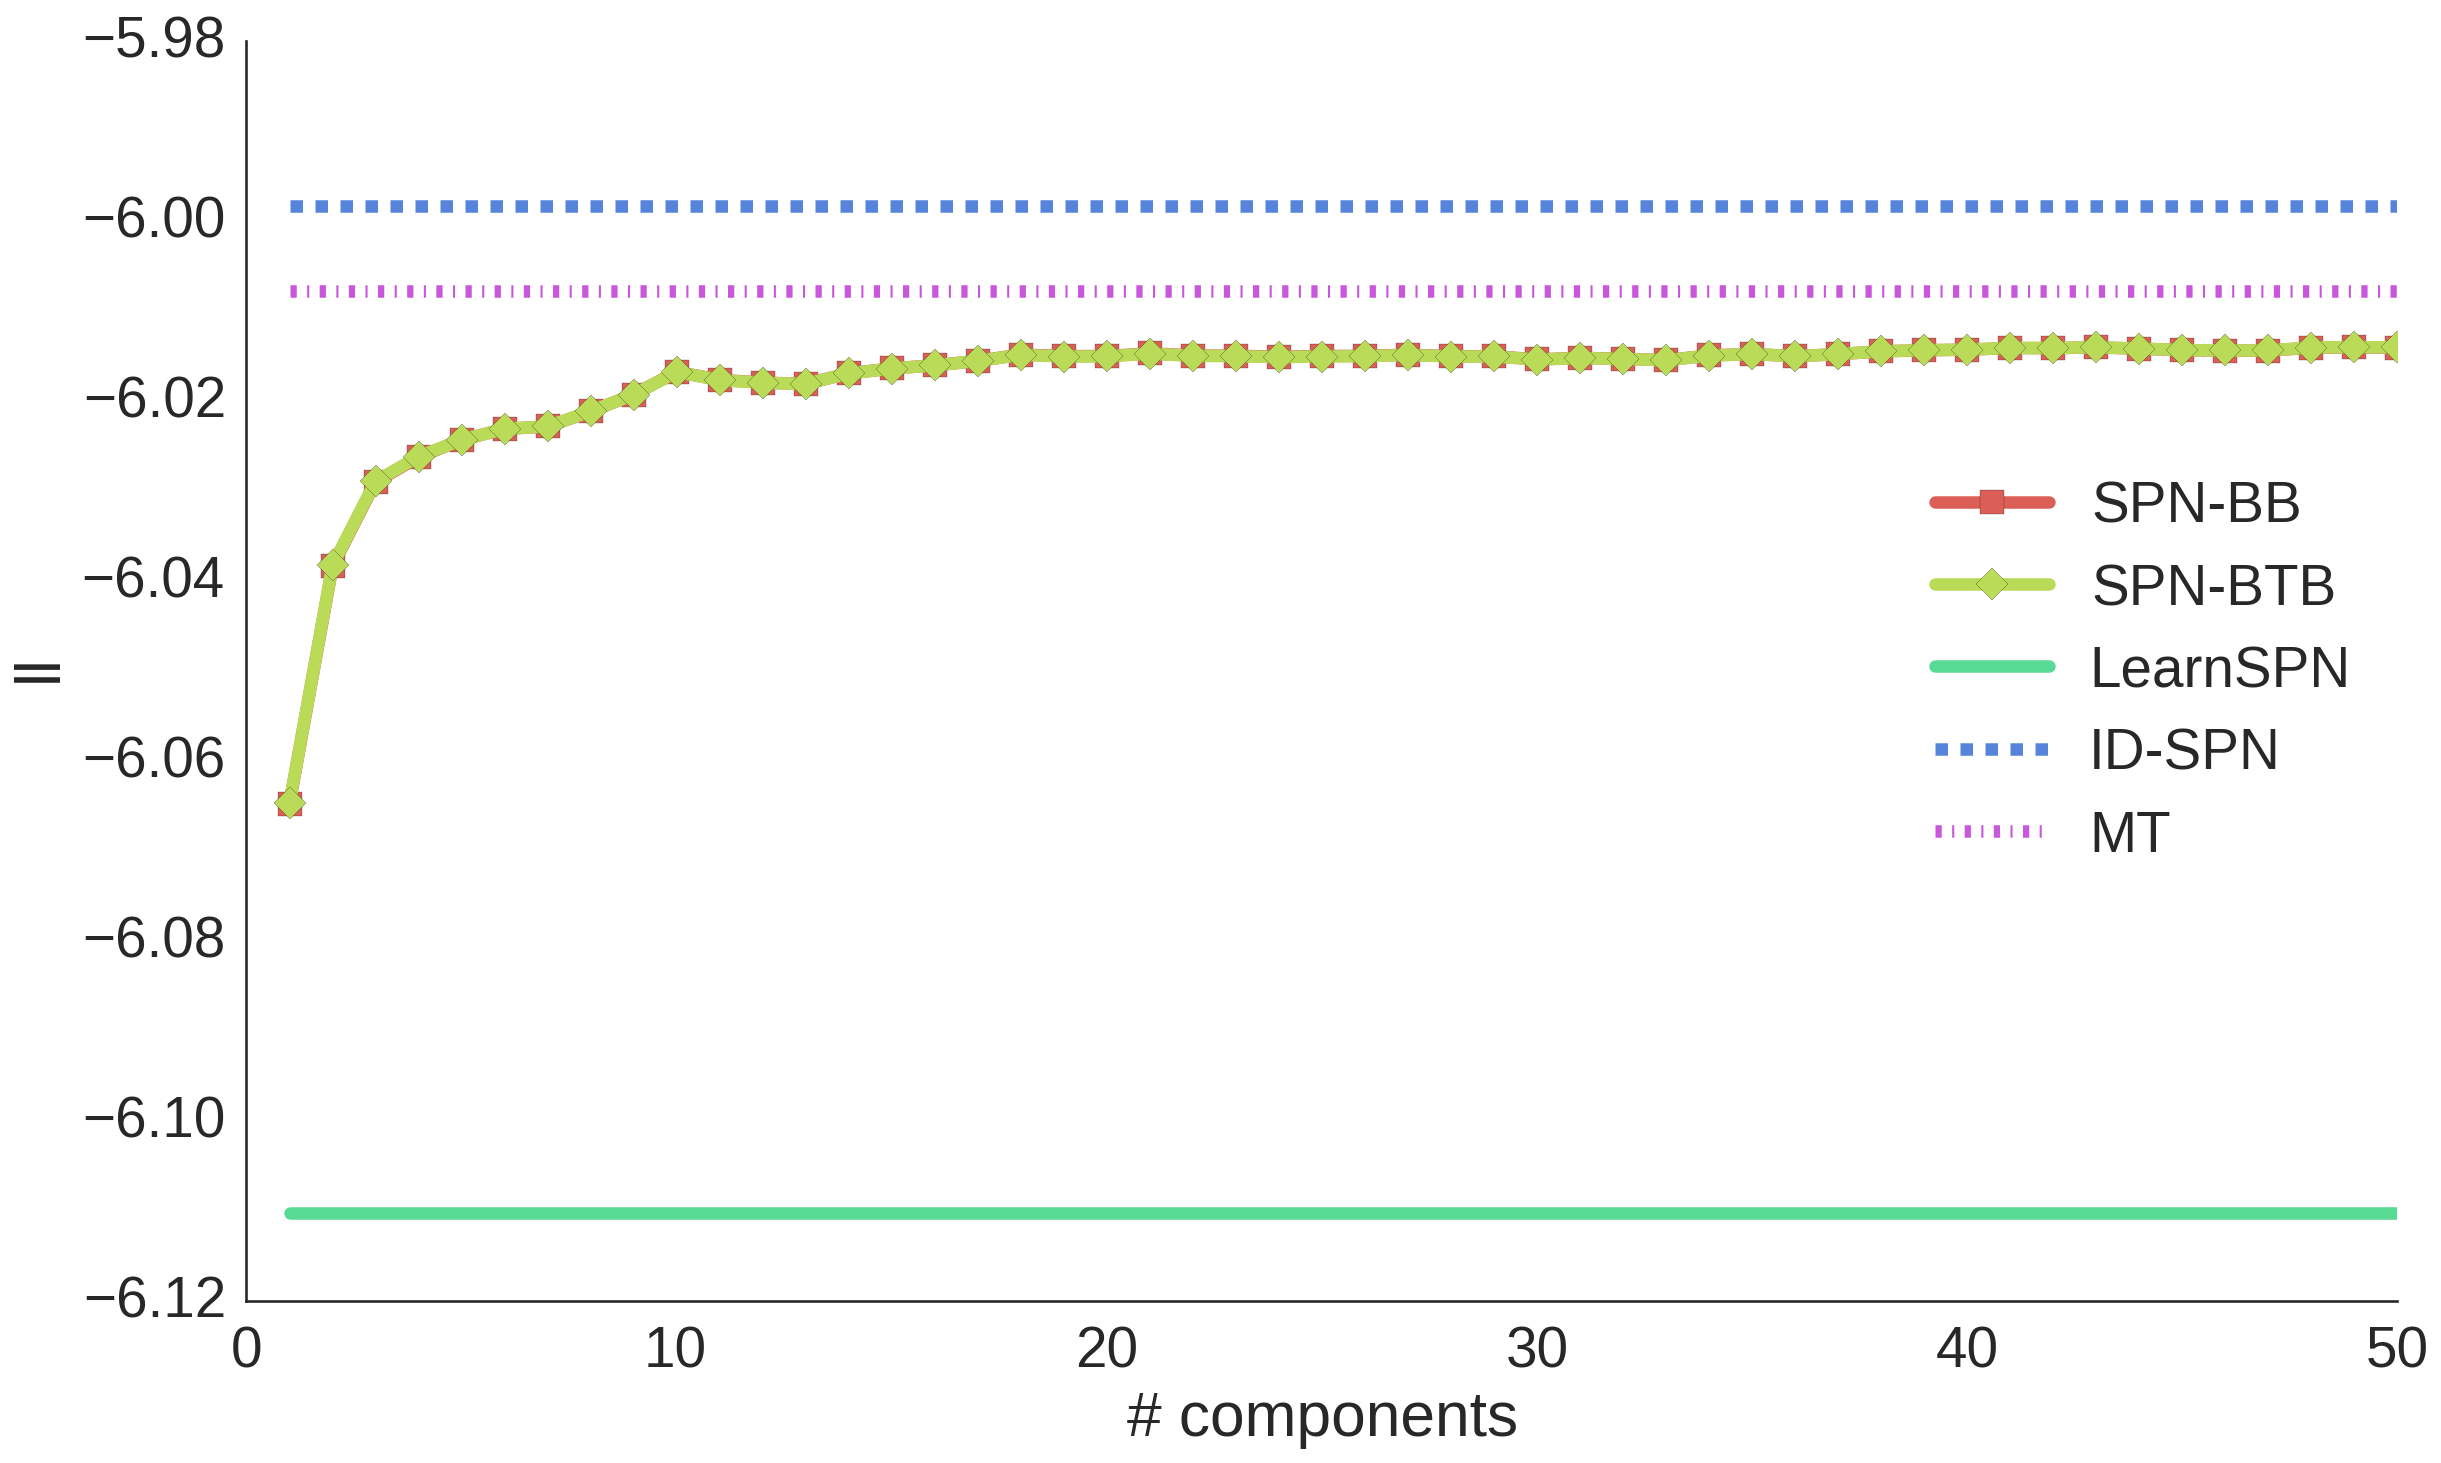
\includegraphics[width=0.4\linewidth]{figures/curves/nltcs}\\
    \end{tabular}
    \caption{Comparing test log-likelihoods for \textsf{SPN-BB} and
      \textsf{SPN-BTB} while increasing the number of components against \textsf{LearnSPN}, \textsf{MT} and
      \textsf{ID-SPN} best models accuracies for Pumsb\_star (left)
      and DNA (right)}
  \end{table}
\end{frame}

\begin{frame}[t]
  \frametitle{Experimental setting}
  \footnotesize
  Classical setting for \emph{\textbf{generative}} PGMs
  structure learning~\emph{\parencite{Gens2013}}:
  \begin{itemize}
    \item 19 binary datasets from classification, recommendation,
    frequent pattern mining\dots~\emph{\parencite{Lowd2010}}~\emph{\parencite{Haaren2012}}
  \item Training 75\% Validation 10\% Test 15\%  splits (no cv)
  \end{itemize}

  Observing both structure quality parameters and the network
  accuracy:
  \begin{itemize}
   \item test set \emph{\textbf{average log-likelihood}}
   \item network \textbf{\emph{size}} (\# edges) and network \textbf{\emph{depth}} (\# levels)
  \end{itemize}
   
  We perform a model selection via a \textit{grid search} in the same parameter
  space for \textsf{LearnSPN}, \textsf{SPN-B}, \textsf{SPN-BT}:\\[-3pt]
  
    \begin{minipage}[t]{0.35\linewidth}
      \begin{itemize}
      \item \scriptsize$\lambda \in \{0.2, 0.4, 0.6, 0.8\}$,
      \item \scriptsize$\rho \in \{5, 10, 15, 20\}$, 
      \end{itemize}
    \end{minipage}\begin{minipage}[t]{0.5\linewidth}
      \begin{itemize}
      \item \scriptsize$m \in \{1, 50, 100, 500\}$, 
      \item \scriptsize$\alpha \in \{ 0.1, 0.2, 0.5, 1.0, 2.0\}$.
      \end{itemize}
    \end{minipage}

    Up to 50 components and best grid parameters for \textsf{SPN-BB} and \textsf{SPN-BTB}.
    Comparing ll against \textsf{LearnSPN},
    \textsf{ID-SPN} and \textsf{MT}~\emph{\parencite{Meila2000}}.

  \end{frame}


  \begin{frame}
    \frametitle{Network sizes}

    \begin{figure}[htbp]
      \begin{center}
        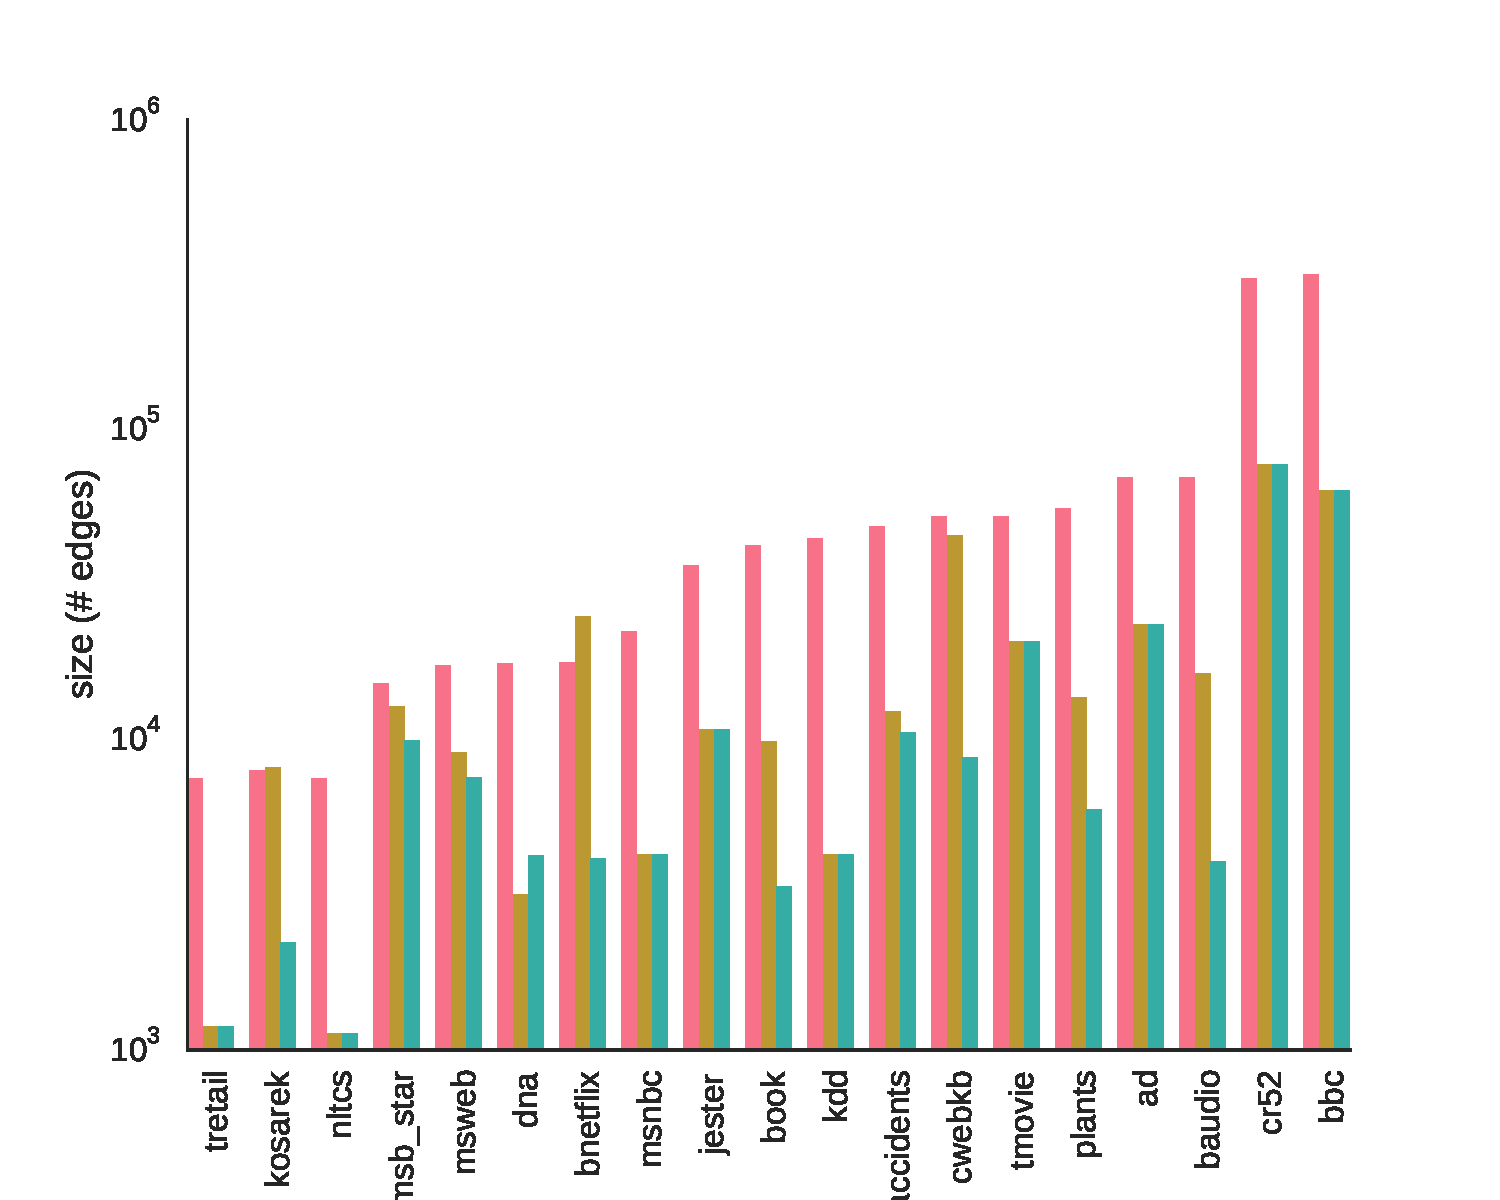
\includegraphics[width=0.65\linewidth]{figures/edges-comp.pdf}
        \caption{Comparing network sizes
          for the networks scoring the best log-likelihoods in the grid
          search as obtained by \textsf{LearnSPN}, \textsf{SPN-B} and
          \textsf{SPN-BT} for each dataset.}
      \end{center}
    \end{figure}
  \end{frame}

  \begin{frame}
    \frametitle{Network depths}

    \begin{figure}[htbp]
      \begin{center}
        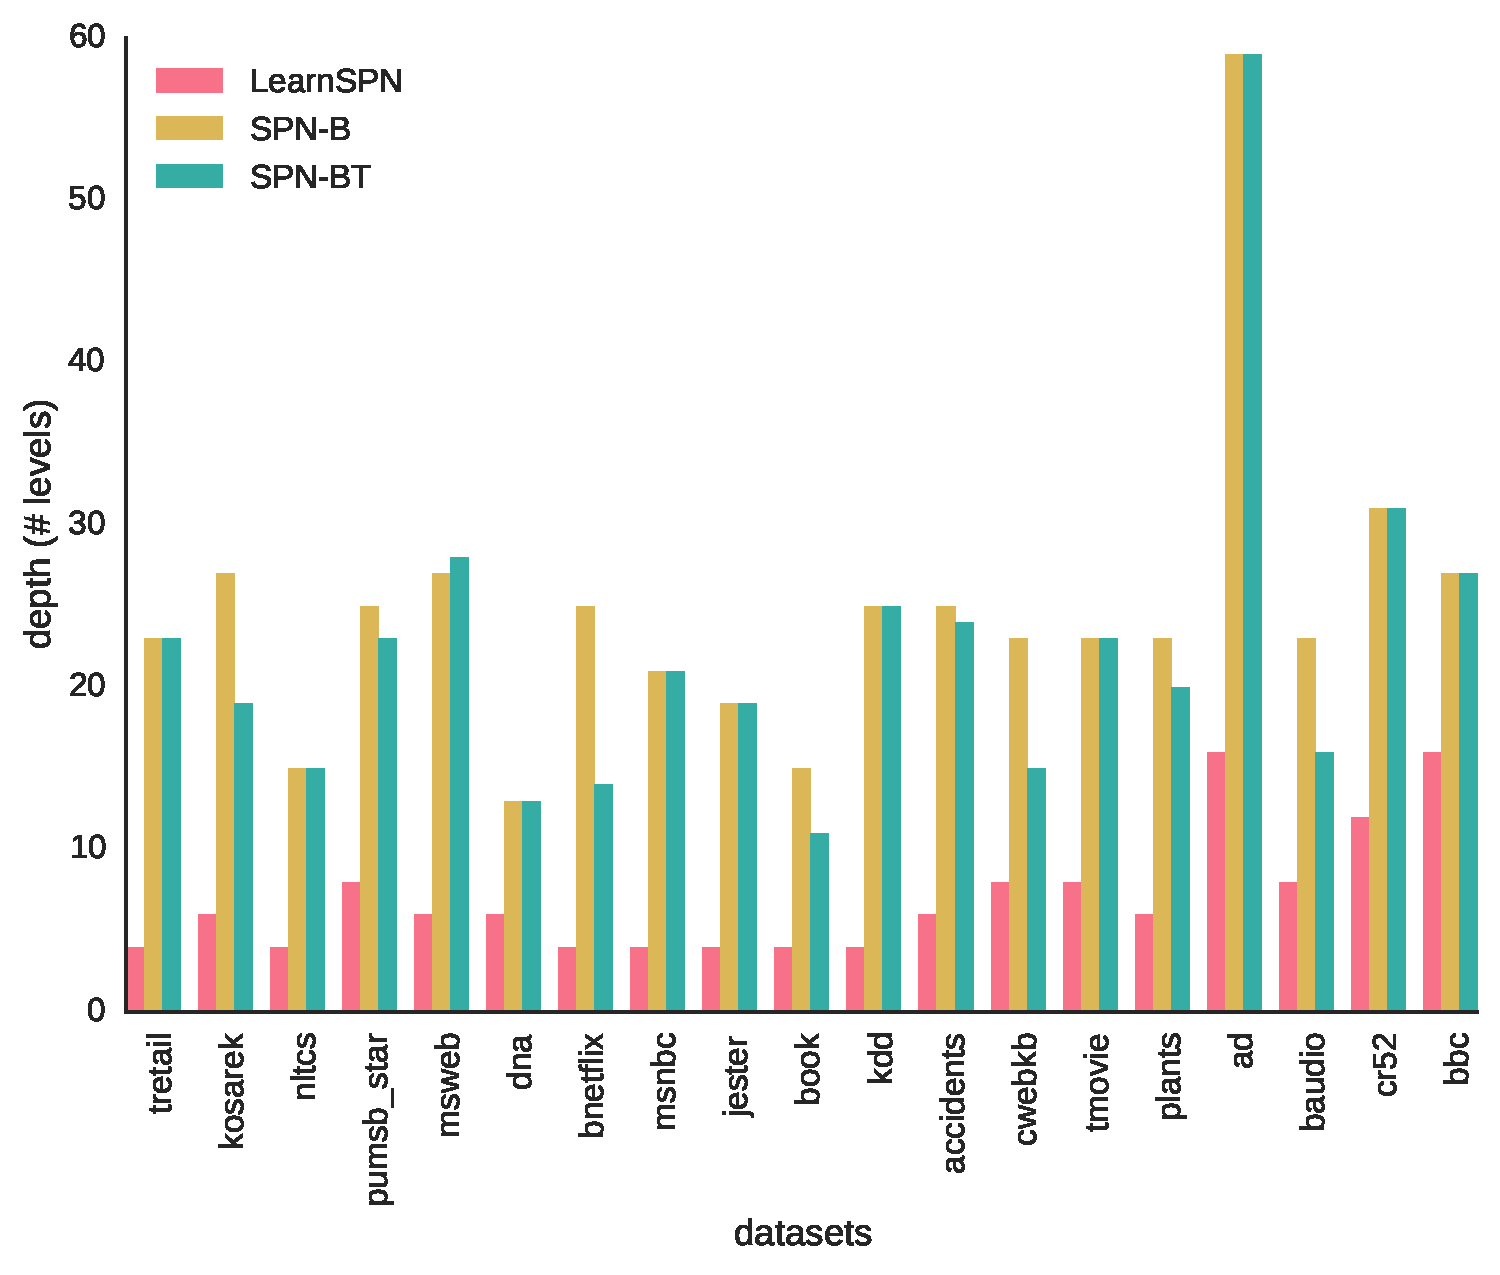
\includegraphics[width=0.65\linewidth]{figures/levels-comp.pdf}
        \caption{Comparing network depths
          for the networks scoring the best log-likelihoods in the grid
          search as obtained by \textsf{LearnSPN}, \textsf{SPN-B} and
          \textsf{SPN-BT} for each dataset.}
      \end{center}
    \end{figure}
  \end{frame}

\begin{frame}
  \frametitle{Log-likelihoods}
  \tiny
  \begin{table}[!htbp]
    \centering
     \setlength{\tabcolsep}{3pt}  
    \begin{tabular}{r r r r r r r r}
      \toprule
      & \textsf{LearnSPN} & \textsf{SPN-B} & \textsf{SPN-BT} & \textsf{ID-SPN}  & \textsf{SPN-BB}   & \textsf{SPN-BTB}  & \textsf{MT}      \\
      \midrule                                                                                     
      \textbf{NLTCS}      & -6.110            & -6.048         & -6.048          & \textbf{-5.998}  & -6.014            & -6.014            & -6.008           \\
      \textbf{MSNBC}      & -6.099            & -6.040         & -6.039          & -6.040           & \textbf{-6.032}   & -6.033            & -6.076           \\
      \textbf{KDDCup2k}   & -2.185            & -2.141         & -2.141          & -2.134           & -2.122            & \textbf{-2.121}   & -2.135           \\
      \textbf{Plants}     & -12.878           & -12.813        & -12.683         & -12.537          & -12.167           & \textbf{-12.089}  & -12.926          \\
      \textbf{Audio}      & -40.360           & -40.571        & -40.484         & -39.794          & -39.685           & \textbf{-39.616}  & -40.142          \\
      \textbf{Jester}     & -53.300           & -53.537        & -53.546         & \textbf{-52.858} & \textbf{-52.873}  & -53.600           & -53.057          \\
      \textbf{Netflix}    & -57.191           & -57.730        & -57.450         & \textbf{-56.355} & -56.610           & \textbf{-56.371}  & -56.706          \\
      \textbf{Accidents}  & -30.490           & -29.342        & -29.265         & \textbf{-26.982} & -28.510           & -28.351           & -29.692          \\
      \textbf{Retail}     & -11.029           & -10.944        & 10.942          & \textbf{-10.846} & -10.858           & -10.858           & \textbf{-10.836} \\
      \textbf{Pumsb-star} & -24.743           & -23.315        & -23.077         & \textbf{-22.405} & -22.866           & -22.664           & -23.702          \\
      \textbf{DNA}        & -80.982           & -81.913        & -81.840         & -81.211          & -80.730           & \textbf{-80.068}  & -85.568          \\
      \textbf{Kosarek}    & -10.894           & -10.719        & -10.685         & -10.599          & -10.690           & \textbf{-10.578}  & -10.615          \\
      \textbf{MSWeb}      & -10.108           & -9.833         & -9.838          & -9.726           & -9.630            & \textbf{-9.614}   & -9.819           \\
      \textbf{Book}       & -34.969           & -34.306        & -34.280         & -34.136          & -34.366           & \textbf{-33.818}  & -34.694          \\
      \textbf{EachMovie}  & -52.615           & -51.368        & -51.388         & -51.512          & \textbf{-50.263}  & \textbf{-50.414}  & -54.513          \\
      \textbf{WebKB}      & -158.164          & -154.283       & -153.911        & -151.838         & -151.341          & \textbf{-149.851} & -157.001         \\
      \textbf{Reuters-52} & -85.414           & -83.349        & -83.361         & -83.346          & \textbf{-81.544}  & -81.587           & -86.531          \\
      % \textbf{20 NewsG}  & -155.218          & -152.846       & -153.072        & -151.467         &                   &                   & -154.367         \\
      \textbf{BBC}        & -249.466          & -247.301       & -247.254        & -248.929         & \textbf{-226.359} & \textbf{-226.560} & -259.962         \\
      \textbf{Ad}         & -19.760           & -16.234        & -15.885         & -19.053          & -13.785           & \textbf{-13.595}  & -16.012          \\
      \bottomrule
    \end{tabular}
    \caption[Experimentation results]{Average test
      log likelihoods for the best networks learned by all
      algorithms on all datasets after the grid search. In bold
      the values that are statistically better than all the others
      according to a Wilcoxon signed rank test with $p$-value of 0.05.}
    \label{tab:resexp}
  \end{table}

\end{frame}


\begin{frame}[t]
  \frametitle{Conclusions}
  \begin{itemize}
  \item Structure quality evaluation matters
  \item Deeper networks by applying a simplicity bias when splitting
  \item Regularized SPNs by introducing Chow-Liu trees as leaves
  \item More robust and accurate SPNs with bootstrapped sum nodes
  \end{itemize}\bigskip

  {\usebeamerfont{frametitle}\usebeamercolor{frametitle}
    Further works}\\[3pt]
  \begin{itemize}
    \item Are other sum node interpretations as gam effective?
  \item Is it possible to compress learned structures?
  \item How these variations influence representation learning?
    \item How can these variations be generalized to other tractable PGMs?
  \end{itemize}
  
\end{frame}

\begin{frame}
  \frametitle{References}
  \setlength\bibitemsep{8pt}
  \printbibliography
\end{frame}

\begin{frame}
  \frametitle{Discuss}
  \begin{minipage}[t][][t]{1.5309cm}
    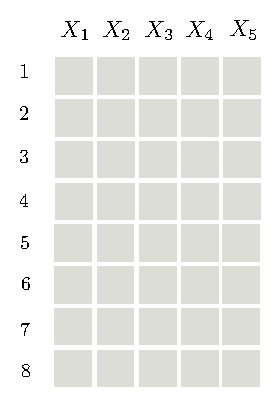
\includegraphics[width=\linewidth]{figures/grid-0}
  \end{minipage}\hspace{10pt}\begin{minipage}[t]{1.3462cm}
    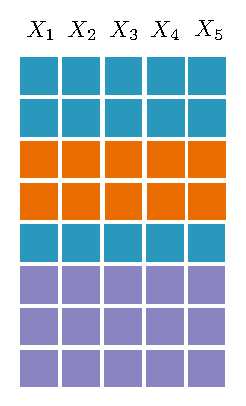
\includegraphics[width=\linewidth]{figures/grid-1}
  \end{minipage}\hspace{10pt}\begin{minipage}[t]{1.3462cm}
    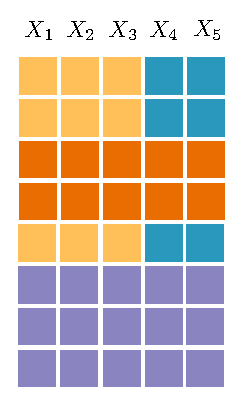
\includegraphics[width=\linewidth]{figures/grid-2}
  \end{minipage}\hspace{10pt}\begin{minipage}[t]{1.3909cm}
    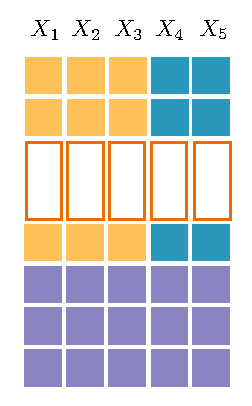
\includegraphics[width=\linewidth]{figures/grid-3}                                                             \end{minipage}

  \begin{minipage}[t]{1.70cm}
      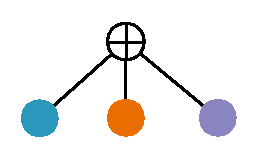
\includegraphics[width=\linewidth]{figures/learnspn-1}
  \end{minipage}\hspace{3pt}\begin{minipage}[t]{2.35cm}
      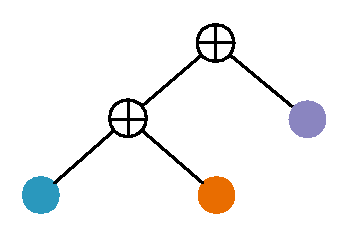
\includegraphics[width=\linewidth]{figures/learnspn-4}
  \end{minipage}\hspace{3pt}\begin{minipage}[t]{2.43cm}
      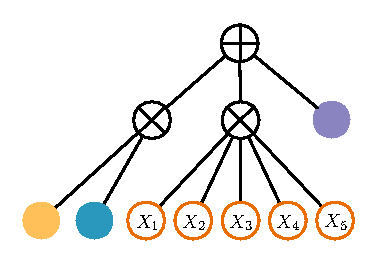
\includegraphics[width=\linewidth]{figures/learnspn-3}                                             
  \end{minipage}\hspace{3pt}\begin{minipage}[t]{2.43cm}
      \includegraphics[width=\linewidth]{figures/spn-clt}                                             
  \end{minipage}\\[-25pt]
  \begin{table}[ht]
    \setlength{\tabcolsep}{3pt}  
    \centering
    \begin{tabular}[t]{c c c c}
      \includegraphics[width=0.23\linewidth]{figures/plants-depth.pdf}&\includegraphics[width=0.23\linewidth]{figures/ll-depth/10-8/pumsb-star-ll-depth}&\includegraphics[width=0.23\linewidth]{figures/ll-m/10-8/pumsb-star-ll-m}&\includegraphics[width=0.23\linewidth]{figures/curves/dna-png.pdf}\\
      % \includegraphics[width=0.4\linewidth]{figures/curves/dna}&\includegraphics[width=0.4\linewidth]{figures/curves/nltcs}\\
    \end{tabular}
  \end{table}      
\end{frame}

\begin{frame}
  \frametitle{Times}
  \begin{table}[htbp]
    \centering
    \tiny
    \setlength{\tabcolsep}{3pt}  
    \begin{tabular}{r r r r r r r r}
      \toprule
      & \textsf{LearnSPN} & \textsf{SPN-B} & \textsf{SPN-BT} & \textsf{ID-SPN} & \textsf{SPN-BB} & \textsf{SPN-BTB} & \textsf{MT} \\
      \midrule                                                                                     
      \textbf{NLTCS}      & 183               & 114            & 108             & 310             & 1004            & 1041             & 290   \\ 
      \textbf{MSNBC}      & 7354              & 5922           & 5774            & 46266           & 7963            & 8275             & 8645  \\ 
      \textbf{KDDCup2k}   & 5800              & 3946           & 4525            & 32067           & 10633           & 12148            & 39857 \\ 
      \textbf{Plants}     & 1156              & 1420           & 276             & 18833           & 7515            & 3023             & 7414  \\ 
      \textbf{Audio}      & 1146              & 1561           & 131             & 21009           & 10466           & 4113             & 6566  \\ 
      \textbf{Jester}     & 1289              & 789            & 687             & 10412           & 17753           & 8566             & 3064  \\ 
      \textbf{Netflix}    & 1331              & 2369           & 152             & 30294           & 14871           & 4768             & 11402 \\ 
      \textbf{Accidents}  & 839               & 1006           & 722             & 15472           & 9198            & 8280             & 14073 \\ 
      \textbf{Retail}     & 253               & 173            & 161             & 4041            & 2317            & 2505             & 320   \\ 
      \textbf{Pumsb-star} & 230               & 1010           & 612             & 20952           & 7819            & 7790             & 18533 \\ 
      \textbf{DNA}        & 140               & 87             & 122             & 3040            & 2022            & 3049             & 228   \\ 
      \textbf{Kosarek}    & 225               & 1515           & 416             & 17799           & 16583           & 3642             & 18782 \\ 
      \textbf{MSWeb}      & 369               & 1711           & 1444            & 19682           & 16881           & 18273            & 36076 \\ 
      \textbf{Book}       & 457               & 832            & 389             & 61248           & 27473           & 16630            & 5918  \\ 
      \textbf{EachMovie}  & 307               & 939            & 946             & 118782          & 22506           & 29355            & 12100 \\ 
      \textbf{WebKB}      & 307               & 1960           & 490             & 45451           & 29265           & 34952            & 931   \\ 
      \textbf{Reuters-52} & 2538              & 5256           & 4333            & 70864           & 36109           & 135970           & 15082 \\ 
      % \textbf{20 NewsG}  & 8897              & 16799          & 13095           & 0               & 13384           & 25156            & 98239\\ 
      \textbf{BBC}        & 1136              & 2645           & 2479            & 61471           & 56271           & 121007           & 1324  \\ 
      \textbf{Ad}         & 668               & 1585           & 1356            & 87522           & 72632           & 58777            & 6850  \\ 
      \bottomrule
    \end{tabular}
    \caption[Experimental times]{Times (in seconds) taken to learn the best
      models on each dataset for \textsf{LearnSPN},
      \textsf{SPN-B}, \textsf{SPN-BT}, \textsf{SPN-BB}, \textsf{SPN-BTB}
      and \textsf{MT} and with default parameters values for
      \textsf{ID-SPN}. Experiments run on a 4-core Intel Xeon E312xx
      (Sandy Bridge) @2.0 GHz with 8Gb of
      RAM and Ubuntu 14.04.1, kernel 3.13.0-39.}
    \label{tab:times}
  \end{table}
\end{frame}

\end{document}

%%% Local Variables:
%%% mode: latex
%%% TeX-master: t
%%% TeX-engine: xetex
%%% End:
